%-------------------------------------------------------------------------------------------%
\pagebreak
\chapter{USABILIDADE DA FERRAMENTA COMPUTACIONAL}\label{sec:userinterface}

Nesta seção apresentam-se detalhes da interface escolhida para facilitar o uso da ferramenta computacional. A interface de usuário foi concebida para permitir o controle de todas as estruturas descritas na Seção~\ref{sec:estrutura} com todos os seus recursos gráficos extraídos. A interface se divide em dois ambientes: um console, que permite uma interação textual e acesso as mesmas funcionalidades de iteração; e uma janela com elementos gráficos capazes de exibir os resultados gráficos obtidos. 

\begin{figure}[!htbp]
	\centering
	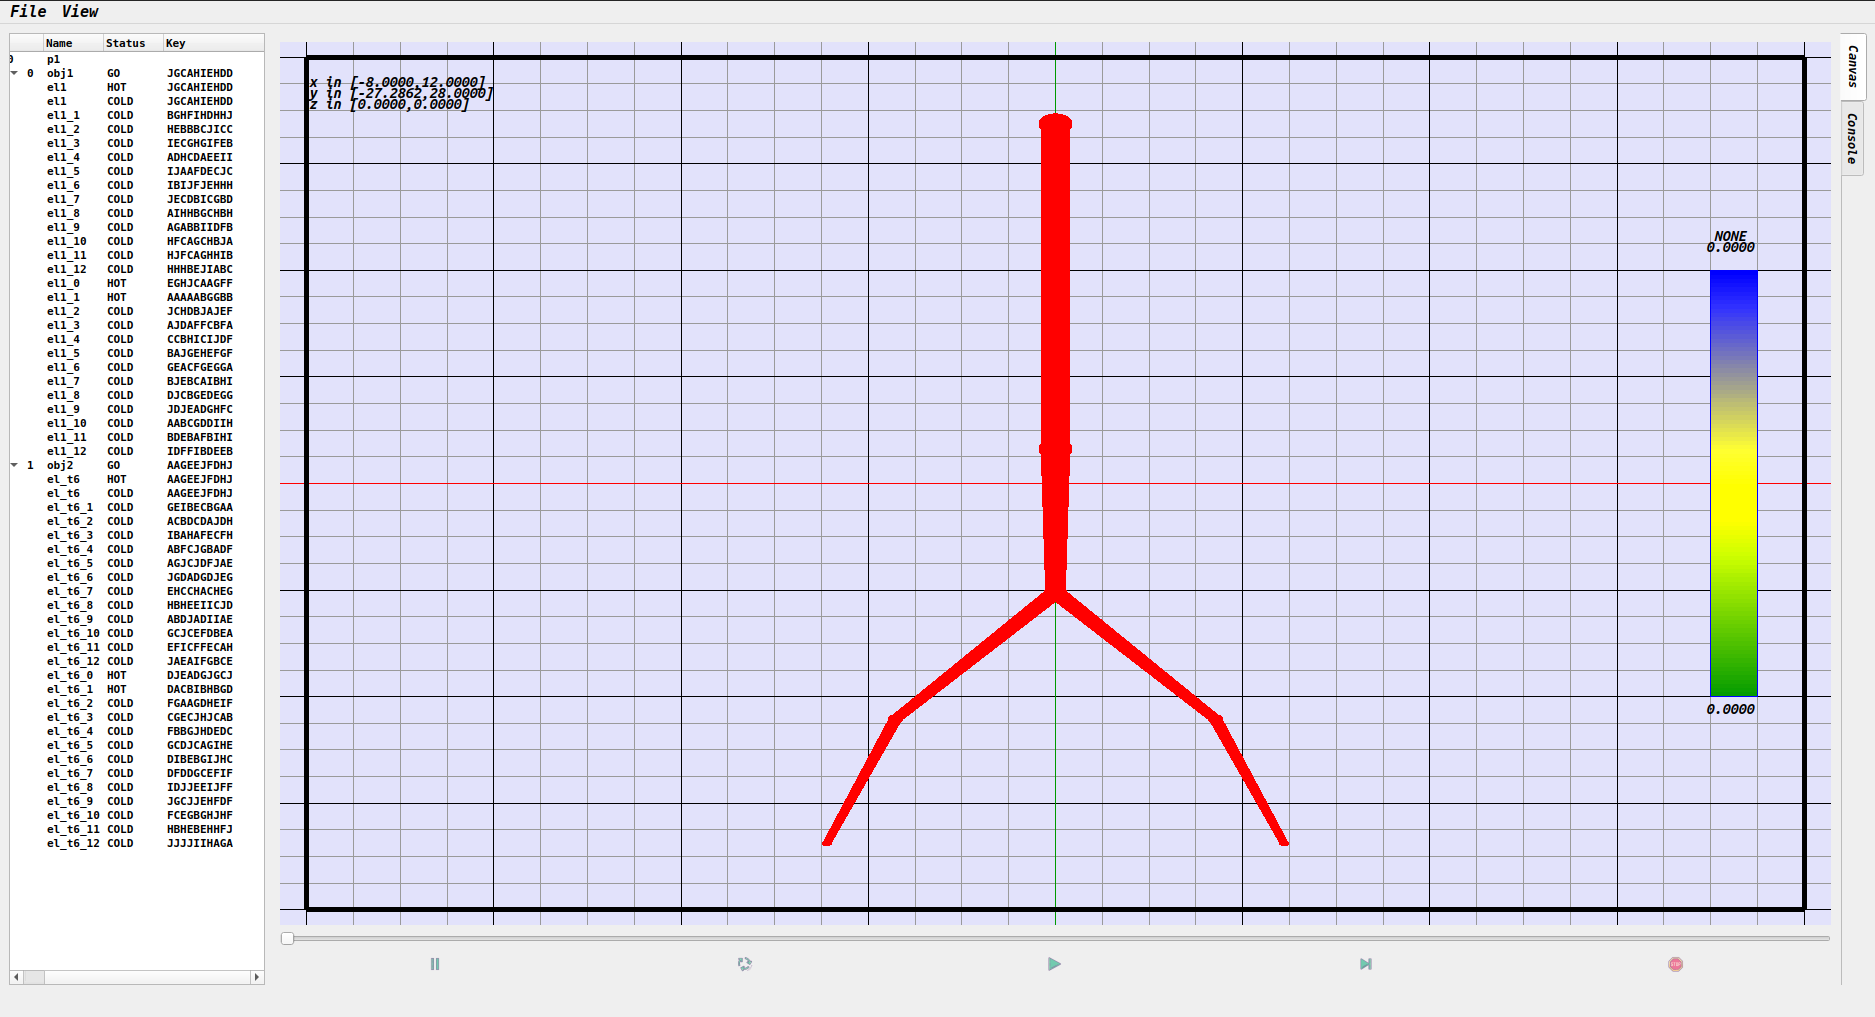
\includegraphics[width=\linewidth]{Figures/IGU_002.png}
	\caption{Ilustração da interface gráfica da ferramenta computacional.}
	\label{fig10:UI}
\end{figure}

Ambas as interfaces foram construídas para manipular objetos e suas estruturas, por isto ambas possuem instâncias do gerenciador de \textit{threads} descritos na Seção~\ref{sec:threads}. O console trata de um envio direto de mensagens para a \textit{thread} \textit{WiseConsole}, que é efetivamente o console. Os diferentes ambientes da ferramenta computacional são descritos. Cada ambiente de interface representa um projeto \textit{Qt}/\textit{C++} distinto e podem utilizar as mesmas classes.

%-------------------------------------------------------------------------------------------%
\section{CONSOLE}\label{sec:console}

O ambiente de console da ferramenta computacional consiste em um projeto \textit{Qt}/\textit{C++} sem interface gráfica. O projeto foi intitulado \textit{InGU} ou \textit{\textbf{I}terador \textbf{n}ão-\textbf{G}ráfico \textbf{U}niversal}, porque o ambiente apesar de não conter os elementos para a visualização dos elementos gráficos, é capaz de criar as estruturas gráficas para visualização futura.  No console, as bibliotecas gráficas do OpenGL não foram incluídas no processo de compilação, portanto ambientes sem recursos gráficos são capazes de compilar e executar a ferramenta computacional através deste ambiente.

\begin{figure}[!htbp]
	\centering
	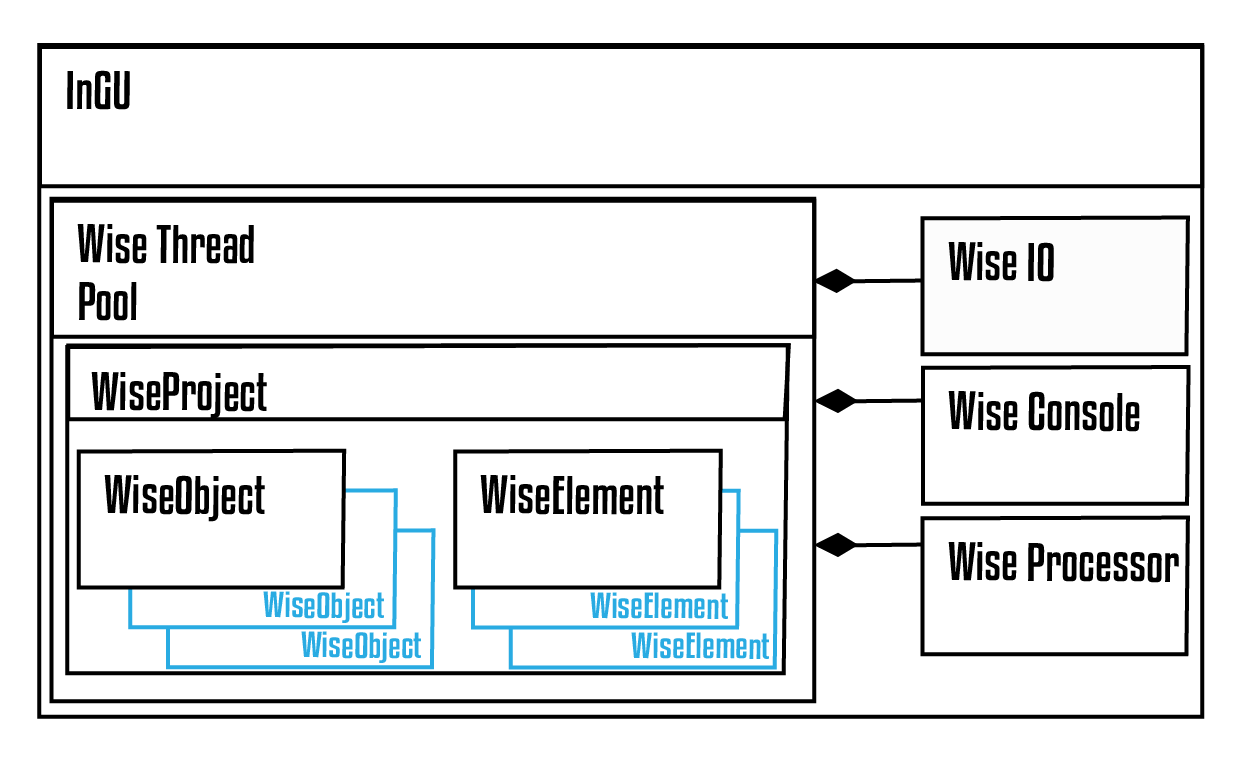
\includegraphics[width=\linewidth]{Figures/InGU.png}
	\caption{Estrutura do projeto que compõe o ambiente computacional \textit{InGU}.}
	\label{fig10:console}
\end{figure}

No Anexo~\ref{annex1} estão as sequências de instruções necessárias para compilar todos os projetos da ferramenta computacional. Ao ser compilado, um executável \textit{InGU} contendo o projeto console é gerado. Ao ser executado, o console padrão do sistema operacional irá ser aberto com o cabeçalho da ferramenta e aguardará entrada de texto.

\begin{figure}[!htbp]
	\centering
	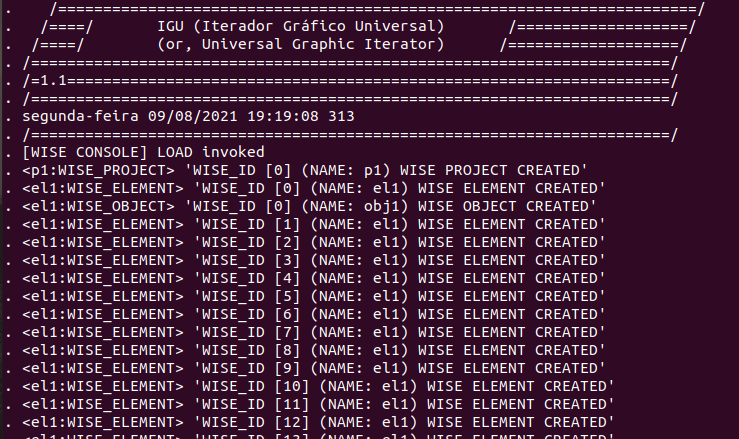
\includegraphics[scale=0.45]{Figures/InGU_console.png}
	\caption{Captura de tela com a execução do ambiente computacional \textit{InGU} em um console.}
	\label{fig11:ajuda}
\end{figure}

Para executar um comando, basta inserir uma linha de texto e apertar a tecla \textit{Enter}.  Ao capturar a linha de texto, o programa de console irá na verdade redirecionar o comando para a estrutura \textit{WiseThreadPool}, que por sua vez irá alocar uma \textit{thread} do tipo \textit{WiseConsole} para interpretar a mensagem. Este comportamento é o mesmo apresentado na Seção~\ref{sec:threads}. Uma lista de comandos foi disponibilizada e está acessível através do comando \textit{help}. Ao enviar este comando para o console, uma lista com todos as possíveis entradas será exibida. Nas próximas seções, estes comandos, suas entradas, seu escopo e \textit{thread} responsável são descritos. Esta \textit{thread} irá executar a tarefa. 

%--------------------------------------------------------------------------------%
\subsection{AJUDA}\label{sec:help}

O comando para ajuda(\textit{help}, Tabela~\ref{tab:help}) é o primeiro comando da interface e foi feito para listar todas as entradas possíveis do programa. Ao receber este comando a thread \textit{WiseConsole} envia o texto pré-definido com todos os comandos.

\begin{center}
	\begin{table}[!htbp]
		\begin{tabularx}{\textwidth}{c|c|X}
			\toprule
			\textbf{Linha de Comando} & \multicolumn{2}{c}{help} \\
			\midrule
			\textbf{Escopo} & \multicolumn{2}{c}{nenhum} \\
			\hline
			\textbf{Thread Responsável} & \multicolumn{2}{c}{\textit{WiseConsole}} \\
			\hline
			\textbf{Entrada} & <vazio> & Nenhuma \\
			\bottomrule
		\end{tabularx}
		\caption{Descrição do comando para ajuda.}
		\label{tab:help}
	\end{table}
\end{center}

Ao executar o comando, o usuário receberá uma lista de comandos divididos em escopos específicos, \igunew{como visto na Figura~\ref{fig10:ajuda}}. Os escopos foram criados para agrupar comandos por área de atuação, comandos auxiliares, como o comando de ajuda, são os comandos que não alteram as estruturas e exibem informações auxiliares ao usuário.


\begin{figure}[!htbp]
	\centering
	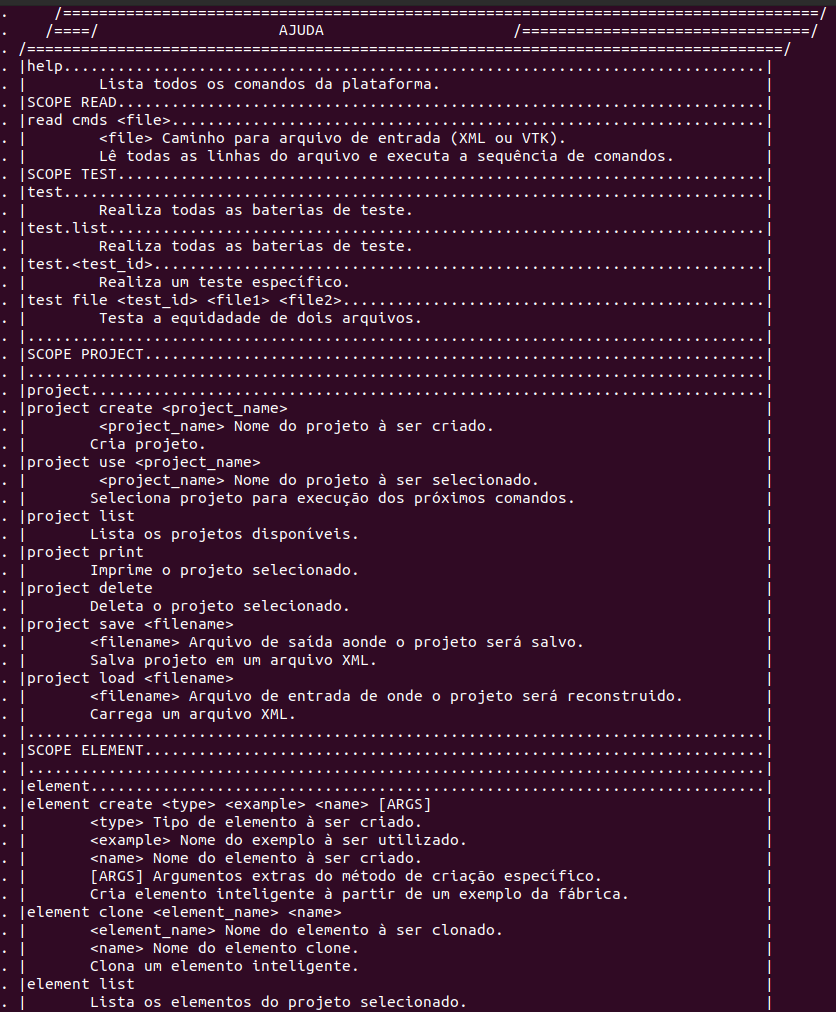
\includegraphics[scale=0.45]{Figures/InGU_help.png}
	\caption{Captura de tela com a execução do comando de ajudo no ambiente computacional \textit{InGU} em um console.}
	\label{fig10:ajuda}
\end{figure}


%--------------------------------------------------------------------------------%
\subsection{LER ARQUIVO DE ENTRADA}\label{sec:read_cmds}


O comando para ler arquivo (Tabela~\ref{tab:read}) irá receber o endereço de um arquivo local, este arquivo deve conter um comando por linha, um exemplo pode ser encontrado no Anexo~\ref{annex2}. Para este tipo de comando, deve-se enviar um \textit{WiseJob} contendo a linha de comando e qual a sequência de trabalhos que será executada. Por se tratar de uma leitura de arquivo de comando, a \textit{thread} \textit{WiseIO} será responsável por ler o arquivo e criar os trabalhos com os comandos subsequentes. Estes novos comandos irão passar novamente pela interpretação de uma \textit{thread} do tipo \textit{WiseConsole} e em seguida executados.

\begin{center}
	\begin{table}[!htbp]
		\begin{tabularx}{\textwidth}{c|c|X}
			\toprule
			\textbf{Linha de Comando} & \multicolumn{2}{c}{read cmds <file>} \\
			\midrule
			\textbf{Escopo} & \multicolumn{2}{c}{READ} \\
			\hline
			\textbf{Thread Responsável} & \multicolumn{2}{c}{\textit{WiseIO}} \\
			\hline
			\textbf{Entrada} & \textbf{<file>} & Caminho para arquivo contendo sequência de comandos \\
			\bottomrule
		\end{tabularx}
		\caption{Descrição do comando para ler arquivo de comando.}
		\label{tab:read}
	\end{table}
\end{center}

%--------------------------------------------------------------------------------%
\subsection{BATERIA DE TESTES}\label{sec:test}

O ciclo principal de testes da ferramenta se baseia em verificar a consistência de todas as fábricas e do fluxo principal da ferramenta computacional, exceto detalhes gráficos e do processo de iteração. Ao executar a bateria de testes todos os elementos \textit{WiseElement} e objetos \textit{WiseObject} disponíveis serão testados individualmente. Para isto, uma fábrica de projeto \textit{WiseProjectFactory} irá ser encarregada de criar todos os elementos e objetos disponíveis.

Estes testes foram utilizados principalmente no momento do desenvolvimento da ferramenta e garantem que as fábricas de elementos e objetos estão funcionando corretamente. Futuramente, caso novas estruturas sejam incluídas, estes testes garantem que todas as classes do projeto foram elaboradas corretamente, com isso todas as estruturas que são carregadas pela ferramenta não perdem informação ao serem armazenadas e recuperadas, processo recorrente na ferramenta computacional. Os comandos deste tipo (Tabela~\ref{tab:test}) são de responsabilidade da \textit{thread} \textit{WiseConsole}, que irá criar e executar trabalhos \textit{WiseJob} correspondente a bateria de testes. Ao finalizar estes trabalhos, os resultados são impressos na tela e o trabalho principal finalizado.

\begin{center}
	\begin{table}[!htbp]
		\begin{tabularx}{\textwidth}{c|c|X}
			\toprule
			\textbf{Linha de Comando} & \multicolumn{2}{c}{test} \\
			\midrule
			\textbf{Escopo} & \multicolumn{2}{c}{TEST} \\
			\hline
			\textbf{Thread Responsável} & \multicolumn{2}{c}{\textit{WiseConsole}} \\
			\hline
			\textbf{Entrada} & <vazio> & Nenhuma \\
			\bottomrule
		\end{tabularx}
		\caption{Descrição do comando para bateria de testes.}
		\label{tab:test}
	\end{table}
\end{center}

%--------------------------------------------------------------------------------%
\subsection{LISTA DE TESTES}\label{sec:test list}

O comando para listar testes (Tabela~\ref{tab:list_test}) irá enumerar todos os testes possíveis de serem executados pela ferramenta computacional. Assim como o comando de ajuda, este comando irá imprimir no console todos os resultados encontrados.

\begin{center}
	\begin{table}[!htbp]
		\begin{tabularx}{\textwidth}{c|c|X}
			\toprule
			\textbf{Linha de Comando} & \multicolumn{2}{c}{test list} \\
			\midrule
			\textbf{Escopo} & \multicolumn{2}{c}{TEST} \\
			\hline
			\textbf{Thread Responsável} & \multicolumn{2}{c}{\textit{WiseConsole}} \\
			\hline
			\textbf{Entrada} & <vazio> & Nenhuma \\
			\bottomrule
		\end{tabularx}
		\caption{Descrição do comando para listar testes.}
		\label{tab:list_test}
	\end{table}
\end{center}

%--------------------------------------------------------------------------------%
\subsection{CASO DE TESTE}\label{sec:case list}

Como mencionado anteriormente, os testes são enumerados. Baseando-se nessa lista, é possível selecionar um teste pelo seu número correspondente utilizando o comando para executar caso de teste (Tabela~\ref{tab:case_test}). Os casos de testes irão gerar uma sequência de comandos a serem interpretados pelo \textit{WiseConsole}. Os testes são compostos de comandos que irão criar e deletar estruturas que são finalizados na própria \textit{thread} \textit{WiseConsole}. Entretanto estas estruturas são enviadas para um arquivo externo e então lidas. Estes subcomandos irão ser executados pela \textit{thread} \textit{WiseIO}. O caso de teste só é dado como concluído quando todos os subcomandos terminam sua execução.

\begin{center}
	\begin{table}[!htbp]
		\begin{tabularx}{\textwidth}{c|c|X}
			\toprule
			\textbf{Linha de Comando} & \multicolumn{2}{c}{test <test\underline{\space}id>} \\
			\midrule
			\textbf{Escopo} & \multicolumn{2}{c}{TEST} \\
			\hline
			\textbf{Thread Responsável} & \multicolumn{2}{c}{\textit{WiseConsole}} \\
			\hline
			\textbf{Entrada} & <test\underline{\space}id> & Número do teste a ser executado \\
			\bottomrule
		\end{tabularx}
		\caption{Descrição do comando para executar caso de teste.}
		\label{tab:case_test}
	\end{table}
\end{center}

%--------------------------------------------------------------------------------%
\subsection{TESTAR IGUALDADE DE ARQUIVOS}\label{sec:test_file}

Outro comando de teste disponibilizado pela ferramenta computacional é o teste de igualdade de arquivos (Tabela~\ref{tab:file_test}). Este comando utiliza uma chave numérica \textit{test\underline{\space}id} para salvar o resultado do teste. Tanto o resultado quanto a quantidade de testes executados com a mesma chave são salvos. Por se tratar da leitura de dois arquivos diferentes esse comando é executado por uma \textit{thread} do tipo \textit{WiseIO}.

\begin{center}
	\begin{table}[!htbp]
		\begin{tabularx}{\textwidth}{c|c|X}
			\toprule
			\textbf{Linha de Comando} & \multicolumn{2}{c}{test file <test\underline{\space\space}id> <file1> <file2>} \\
			\midrule
			\textbf{Escopo} & \multicolumn{2}{c}{TEST} \\
			\hline
			\textbf{Thread Responsável} & \multicolumn{2}{c}{\textit{WiseIO}} \\
			\hline
			\multirow{3}{*}{\textbf{Entrada}} & <test\underline{\space\space}id> & Chave numérica para armazenar resultado \\
			& <file1> & Caminho para o primeiro arquivo \\
			& <file2> & Caminho para o segundo arquivo \\
			\bottomrule
		\end{tabularx}
		\caption{Descrição do comando para testar a igualdade de dois arquivos.}
		\label{tab:file_test}
	\end{table}
\end{center}

%--------------------------------------------------------------------------------%
\subsection{CRIAR PROJETO}\label{sec:create_projects}

Comando utilizado para criar um novo projeto (Tabela~\ref{tab:create_project}), o qual recebe como entrada o nome do projeto. Este comando irá utilizar a fábrica de projetos para criar a estrutura vazia do projeto. Ao receber um comando deste a \textit{thread} \textit{WiseConsole} irá retornar um projeto em branco para ser acoplado à \textit{WiseThreadPool}. Isto é feito para que outras \textit{threads} possam receber o mesmo projeto de forma separada.

\begin{center}
	\begin{table}[!htbp]
		\begin{tabularx}{\textwidth}{c|c|X}
			\toprule
			\textbf{Linha de Comando} & \multicolumn{2}{c}{project create <name>} \\
			\midrule
			\textbf{Escopo} & \multicolumn{2}{c}{PROJECT} \\
			\hline
			\textbf{Thread Responsável} & \multicolumn{2}{c}{WiseConsole} \\
			\hline
			\textbf{Entrada} & <name> & Nome do projeto a ser criado \\
			\bottomrule
		\end{tabularx}
		\caption{Descrição do comando para criar projetos.}
		\label{tab:create_project}
	\end{table}
\end{center}

%--------------------------------------------------------------------------------%
\subsection{USAR PROJETO}\label{sec:use_projects}

Para que a maioria dos comandos funcione é necessário que um projeto esteja selecionado, pois é a estrutura do projeto que disponibiliza elementos e objetos. Uma vez que projetos tenham sido criados, eles podem ser selecionados utilizando o comando para usar projetos (Tabela~\ref{tab:use_project}).

\begin{center}
	\begin{table}[!htbp]
		\begin{tabularx}{\textwidth}{c|c|X}
			\toprule
			\textbf{Linha de Comando} & \multicolumn{2}{c}{project use <project\underline{\space\space}name>} \\
			\midrule
			\textbf{Escopo} & \multicolumn{2}{c}{PROJECT} \\
			\hline
			\textbf{Thread Responsável} & \multicolumn{2}{c}{\textit{WiseConsole}} \\
			\hline
			\textbf{Entrada} & <project\underline{\space\space}name> & Nome do projeto a ser selecionado \\
			\bottomrule
		\end{tabularx}
		\caption{Descrição do comando para selecionar projetos.}
		\label{tab:use_project}
	\end{table}
\end{center}

%--------------------------------------------------------------------------------%
\subsection{LISTAR PROJETOS}\label{sec:list_projects}

É possível verificar todos os projetos do ambiente utilizando o comando para listar projetos (Tabela~\ref{tab:list_project}). Todos os projetos carregados no momento da execução são exibidos na listagem.

\begin{center}
	\begin{table}[!htbp]
		\begin{tabularx}{\textwidth}{c|c|X}
			\toprule
			\textbf{Linha de Comando} & \multicolumn{2}{c}{project list} \\
			\midrule
			\textbf{Escopo} & \multicolumn{2}{c}{PROJECT} \\
			\hline
			\textbf{Thread Responsável} & \multicolumn{2}{c}{\textit{WiseConsole}} \\
			\hline
			\textbf{Entrada} & <vazio> & Nenhuma \\
			\bottomrule
		\end{tabularx}
		\caption{Descrição do comando para listar projetos.}
		\label{tab:list_project}
	\end{table}
\end{center}

%--------------------------------------------------------------------------------%
\subsection{IMPRIMIR PROJETO}\label{sec:print_projects}

\igunew{O comando para imprimir projetos (Tabela~\ref{tab:print_projects}) irá exibir no console a representação do arquivo \textit{XML} do projeto selecionado.} Caso o projeto possua elementos e objetos eles também são impressos na estrutura de saída.

\begin{center}
	\begin{table}[!htbp]
		\begin{tabularx}{\textwidth}{c|c|X}
			\toprule
			\textbf{Linha de Comando} & \multicolumn{2}{c}{project print} \\
			\midrule
			\textbf{Escopo} & \multicolumn{2}{c}{PROJECT} \\
			\hline
			\textbf{Thread Responsável} & \multicolumn{2}{c}{WiseConsole} \\
			\hline
			\textbf{Entrada} & <vazio> & Nenhuma \\
			\bottomrule
		\end{tabularx}
		\caption{Descrição do comando imprimir projetos.}
		\label{tab:print_projects}
	\end{table}
\end{center}

%--------------------------------------------------------------------------------%
\subsection{EXCLUIR PROJETO}\label{sec:delete_projects}

Com um projeto selecionado, o comando para exclusão de elementos (Tabela~\ref{tab:delete_projects}) irá excluir o elemento do projeto recebendo o nome do elemento como parâmetro de entrada. Este comando será interpretado pela \textit{thread} \textit{WiseConsole}, que notifica o gerenciador de \textit{threads} \textit{WiseThreadPool}. O gerenciador só irá aguardar até que o projeto não possua trabalhos em execução para que posso excluí-lo.

\begin{center}
	\begin{table}[!htbp]
		\begin{tabularx}{\textwidth}{c|c|X}
			\toprule
			\textbf{Linha de Comando} & \multicolumn{2}{c}{project delete} \\
			\midrule
			\textbf{Escopo} & \multicolumn{2}{c}{PROJECT} \\
			\hline
			\textbf{Thread Responsável} & \multicolumn{2}{c}{\textit{WiseConsole}} \\
			\hline
			\textbf{Entrada} & <vazio> & Nenhuma \\
			\bottomrule
		\end{tabularx}
		\caption{Descrição do comando para excluir projetos.}
		\label{tab:delete_projects}
	\end{table}
\end{center}

%--------------------------------------------------------------------------------%
\subsection{SALVAR PROJETO}\label{sec:save_projects}

O comando para salvar projetos (Tabela~\ref{tab:save_project}) irá extrair do projeto selecionado sua representação em um arquivo \textit{XML}, assim como no processo de impressão do projeto. Este arquivo será impresso em um arquivo externo e por isto é executado pela thread \textit{WiseIO}.

\begin{center}
	\begin{table}[!htbp]
		\begin{tabularx}{\textwidth}{c|c|X}
			\toprule
			\textbf{Linha de Comando} & \multicolumn{2}{c}{project save <file\underline{\space\space}name>} \\
			\midrule
			\textbf{Escopo} & \multicolumn{2}{c}{PROJECT} \\
			\hline
			\textbf{Thread Responsável} & \multicolumn{2}{c}{\textit{WiseIO}} \\
			\hline
			\textbf{Entrada} & <file\underline{\space\space}name> & Caminho do arquivo de saída \\
			\bottomrule
		\end{tabularx}
		\caption{Descrição do comando para salvar projetos.}
		\label{tab:save_project}
	\end{table}
\end{center}

%--------------------------------------------------------------------------------%
\subsection{CARREGAR PROJETO}\label{sec:load_projects}

O comando para carregar projetos (Tabela~\ref{tab:load_project}) irá extrair de um arquivo de entrada no formato \textit{XML} a estrutura de um projeto. A ferramenta computacional irá utilizar os arquivos de entrada diretamente nas estruturas de fábrica relacionadas. Caso o projeto possua elementos e objetos eles também serão reconstruídos no projeto reconstruído.

\begin{center}
	\begin{table}[!htbp]
		\begin{tabularx}{\textwidth}{c|c|X}
			\toprule
			\textbf{Linha de Comando} & \multicolumn{2}{c}{project load <filename>} \\
			\midrule
			\textbf{Escopo} & \multicolumn{2}{c}{PROJECT} \\
			\hline
			\textbf{Thread Responsável} & \multicolumn{2}{c}{\textit{WiseIO}} \\
			\hline
			\textbf{Entrada} & <filename> & Caminho do arquivo de entrada \\
			\bottomrule
		\end{tabularx}
		\caption{Descrição do comando para carregar projetos.}
		\label{tab:load_project}
	\end{table}
\end{center}

%--------------------------------------------------------------------------------%
\subsection{CRIAR ELEMENTO}\label{sec:create_element}

As fábricas de elementos descritas na Seção~\ref{sec:fabrica} são acessadas pelo comando de criar elementos. Este comando recebe como entrada o tipo de elemento, o nome e o exemplo a ser utilizado. Cada fábrica de elementos possui uma lista de exemplos disponíveis, que é visualizada através do comando para listar exemplos de uma fábrica de elementos (Tabela~\ref{tab:create_element}).

\begin{center}
	\begin{table}[!htbp]
		\begin{tabularx}{\textwidth}{c|c|X}
			\toprule
			\textbf{Linha de Comando} & \multicolumn{2}{c}{element create <type> <example> <name> [ARGS]} \\
			\midrule
			\textbf{Escopo} & \multicolumn{2}{c}{ELEMENT} \\
			\hline
			\textbf{Thread Responsável} & \multicolumn{2}{c}{\textit{WiseConsole}} \\
			\hline
			\multirow{4}{*}{\textbf{Entrada}} & <type> & Tipo de elemento à ser criado, seleciona a fábrica de elemento à ser utilizada. \\
			
			& <example> & Caminho para o primeiro arquivo \\
			& <name> & Caminho para o segundo arquivo \\
			& [ARGS] & Individualmente,  as fábricas podem receber parâmetros para a criação de elementos \\
			\bottomrule
		\end{tabularx}
		\caption{Descrição do comando para criar.}
		\label{tab:create_element}
	\end{table}
\end{center}

%--------------------------------------------------------------------------------%
\subsection{CLONAR ELEMENTO}\label{sec:clone_element}

Assim como o comando para criação de elementos descrito na Seção~\ref{sec:create_element}, ao comando para clonagem de elementos (Tabela~\ref{tab:clone_element}) também irá acessar as fábricas de elementos. Ao clonar um elemento, o seu tipo é selecionado juntamente com a fábrica correspondente. Após serem selecionados a fábrica receberá como parâmetro o elemento e o nome do novo elemento a ser criado. Portanto, o comando de clonagem de elementos poderá ser utilizando com a entrada do nome do elemento a ser clonado e o nome do novo elemento.

\begin{center}
	\begin{table}[!htbp]
		\begin{tabularx}{\textwidth}{c|c|X}
			\toprule
			\textbf{Linha de Comando} & \multicolumn{2}{c}{element clone <element\underline{\space\space}name> <name>} \\
			\midrule
			\textbf{Escopo} & \multicolumn{2}{c}{ELEMENT} \\
			\hline
			\textbf{Thread Responsável} & \multicolumn{2}{c}{\textit{WiseConsole}} \\
			\hline
			\multirow{2}{*}{\textbf{Entrada}} & <element\underline{\space\space}name> & Nome do elemento a ser clonado. \\
			
			& <name> & Nome do novo elemento. \\
			\bottomrule
		\end{tabularx}
		\caption{Descrição do comando para clonar elementos.}
		\label{tab:clone_element}
	\end{table}
\end{center}

%--------------------------------------------------------------------------------%
\subsection{LISTAR ELEMENTOS}\label{sec:list_element}

Com um projeto já selecionado, o comando para listar elementos (Tabela~\ref{tab:list_element}) pode ser utilizado para que o console imprima uma lista com o nome de todos os elementos presentes no projeto.

\begin{center}
	\begin{table}[!htbp]
		\begin{tabularx}{\textwidth}{c|c|X}
			\toprule
			\textbf{Linha de Comando} & \multicolumn{2}{c}{element list} \\
			\midrule
			\textbf{Escopo} & \multicolumn{2}{c}{ELEMENT} \\
			\hline
			\textbf{Thread Responsável} & \multicolumn{2}{c}{\textit{WiseConsole}} \\
			\hline
			\textbf{Entrada} & <vazio> & Nenhuma \\
			\bottomrule
		\end{tabularx}
		\caption{Descrição do comando para listar elementos.}
		\label{tab:list_element}
	\end{table}
\end{center}

%--------------------------------------------------------------------------------%
\subsection{IMPRIMIR ELEMENTO}\label{sec:print_element}

O comando para imprimir elementos (Tabela~\ref{tab:print_element}) irá extrair do projeto selecionado a representação em um arquivo \textit{XML}. A informação textual deste arquivo será impressa como resultado no console. Para que o comando funcione é necessário que um projeto esteja selecionado e que o nome do elemento a ser impresso seja informado.

\begin{center}
	\begin{table}[!htbp]
		\begin{tabularx}{\textwidth}{c|c|X}
			\toprule
			\textbf{Linha de Comando} & \multicolumn{2}{c}{element print <element\underline{\space\space}name>} \\
			\midrule
			\textbf{Escopo} & \multicolumn{2}{c}{ELEMENT} \\
			\hline
			\textbf{Thread Responsável} & \multicolumn{2}{c}{\textit{WiseConsole}} \\
			\hline
			\textbf{Entrada} & <element\underline{\space\space}name> & Nome do elemento à ser impresso \\
			\bottomrule
		\end{tabularx}
		\caption{Descrição do comando para imprimir elementos.}
		\label{tab:print_element}
	\end{table}
\end{center}

%--------------------------------------------------------------------------------%
\subsection{EXCLUIR ELEMENTO}\label{sec:delete_element}

O comando para excluir elementos (Tabela~\ref{tab:delete_element}) irá remover os dados do elemento da memória.

\begin{center}
	\begin{table}[!htbp]
		\begin{tabularx}{\textwidth}{c|c|X}
			\toprule
			\textbf{Linha de Comando} & \multicolumn{2}{c}{element delete <element\underline{\space\space}name>} \\
			\midrule
			\textbf{Escopo} & \multicolumn{2}{c}{ELEMENT} \\
			\hline
			\textbf{Thread Responsável} & \multicolumn{2}{c}{\textit{WiseConsole}} \\
			\hline
			\textbf{Entrada} & <element\underline{\space\space}name> & Nome do elemento a ser excluído. \\
			\bottomrule
		\end{tabularx}
		\caption{Descrição do comando para excluir elementos.}
		\label{tab:delete_element}
	\end{table}
\end{center}

%--------------------------------------------------------------------------------%
\subsection{SALVAR ELEMENTO}\label{sec:save_element}

Os elementos podem ser exportados em dois formatos, um arquivo \textit{XML} e um arquivo \textit{VTK}. Ambos futuramente podem ser utilizados na reconstrução do elemento. Como entrada o comando para salvar elementos (Tabela~\ref{tab:save_element}) receberá o nome do elemento, o tipo de arquivo a ser escrito e o caminho onde ele deve ser salvo. A saída do comando será o arquivo determinado, que a partir dele é possível reconstruir o elemento completo.

\begin{center}
	\begin{table}[!htbp]
		\begin{tabularx}{\textwidth}{c|c|X}
			\toprule
			\textbf{Linha de Comando} & \multicolumn{2}{c}{element save <element\underline{\space\space}name> <save\underline{\space\space}type> <filename>} \\
			\midrule
			\textbf{Escopo} & \multicolumn{2}{c}{ELEMENT} \\
			\hline
			\textbf{Thread Responsável} & \multicolumn{2}{c}{\textit{WiseIO}} \\
			\hline
			\multirow{3}{*}{\textbf{Entrada}} & <element\underline{\space\space}name> & Nome do elemento inteligente a ser salvo. \\
			& <save\underline{\space\space}type> & Tipo de arquivo a ser exportando, podendo ser \textit{XML} ou \textit{VTK} \\
			& <filename> & Caminho para o arquivo a ser exportado \\
			\bottomrule
		\end{tabularx}
		\caption{Descrição do comando para salvar elementos.}
		\label{tab:save_element}
	\end{table}
\end{center}

%--------------------------------------------------------------------------------%
\subsection{CARREGAR ELEMENTO}\label{sec:load_element}

O comando para carregar elemento (Tabela~\ref{tab:load_element}) irá extrair de um arquivo de entrada no formato \textit{XML} ou \textit{VTK} a estrutura de um elemento. A ferramenta computacional irá utilizar os arquivos de entrada diretamente na fábrica de elemento relacionada. Caso seja um arquivo \textit{XML} não será necessário informar o tipo de elemento a ser construído. Caso contrário, o tipo e o nome são recebidos como parâmetros de entrada.

\begin{center}
	\begin{table}[!htbp]
		\begin{tabularx}{\textwidth}{c|c|X}
			\toprule
			\multirow{3}{*}{\textbf{Linha de Comando}} & \multicolumn{2}{c}{element load <load\underline{\space\space}type>} \\
			& \multicolumn{2}{c}{element load <\textbf{VTK}> <filename> <type> <name>} \\
			& \multicolumn{2}{c}{element load <\textbf{XML}> <filename>} \\
			\midrule
			\textbf{Escopo} & \multicolumn{2}{c}{ELEMENT} \\
			\hline
			\textbf{Thread Responsável} & \multicolumn{2}{c}{\textit{WiseIO}} \\
			\hline
			\multirow{3}{*}{\textbf{Entrada}} & <filename> & Caminho para o arquivo de entrada \\
			& <load\underline{\space\space}type> & Tipo de arquivo a ser carregado, podendo ser \textit{XML} ou \textit{VTK} \\
			& <type> & Tipo de elemento a ser criado \\
			& <name> & Nome do elemento a ser criado \\
			\bottomrule
		\end{tabularx}
		\caption{Descrição do comando para carregar elementos.}
		\label{tab:load_element}
	\end{table}
\end{center}

%--------------------------------------------------------------------------------%
\subsection{LISTAR EXPORTAÇÕES DO ELEMENTO}\label{sec:export_list_element}

Os elementos podem ser exportados para outros formatos de arquivo\igunew{, como uma imagem \textit{PNG}, imagem \textit{JPG} ou texto \textit{TXT}}. Cada tipo de elemento possui uma lista de exportações disponíveis. Assim, um comando (Tabela~\ref{tab:export_list_element}) foi inserido para acessar a lista de exportações de um certo objeto.

\begin{center}
	\begin{table}[!htbp]
		\begin{tabularx}{\textwidth}{c|c|X}
			\toprule
			\textbf{Linha de Comando} & \multicolumn{2}{c}{element export\underline{\space\space}list <element\underline{\space\space}name>}  \\
			\midrule
			\textbf{Escopo} & \multicolumn{2}{c}{ELEMENT} \\
			\hline
			\textbf{Thread Responsável} & \multicolumn{2}{c}{\textit{WiseConsole}} \\
			\hline
			\textbf{Entrada} & <element\underline{\space\space}name> & Nome do elemento à analisado \\
			\bottomrule
		\end{tabularx}
		\caption{Descrição do comando para listar exportações de um elemento.}
		\label{tab:export_list_element}
	\end{table}
\end{center}

%--------------------------------------------------------------------------------%
\subsection{EXPORTAR ELEMENTO}\label{sec:export_element}

A estrutura abstrata dos elementos requer que cada um deles possua o método de exportação, este método pode ser utilizado através do comando de exportar elementos (Tabela~\ref{tab:export}). Salienta-se que os métodos de exportação podem receber parâmetros diferentes. A principal exportação utilizada foi disponibilizada na classe \textit{WiseGraphic}, que propicia a exportação dos gráficos em arquivos de imagem. Desta forma, possibilitou-se a criação de imagens em um ambiente que não possui interface gráfica.

\begin{center}
	\begin{table}[!htbp]
		\begin{tabularx}{\textwidth}{c|c|X}
			\toprule
			\textbf{Linha de Comando} & \multicolumn{2}{c}{element export <element\underline{\space\space}name> <export\underline{\space\space}name> [ARGS]} \\
			\midrule
			\textbf{Escopo} & \multicolumn{2}{c}{ELEMENT} \\
			\hline
			\textbf{Thread Responsável} & \multicolumn{2}{c}{\textit{WiseIO}} \\
			\hline
			\multirow{3}{*}{\textbf{Entrada}} & <element\underline{\space\space}name> & Nome do elemento a ser exportado \\
			& <export\underline{\space\space}name> & Tipo de exportação a ser realizada \\
			& [ARGS] & Os elementos podem receber parâmetros para sua exportação \\
			\bottomrule
		\end{tabularx}
		\caption{Descrição do comando para exportar elementos.}
		\label{tab:export}
	\end{table}
\end{center}

%--------------------------------------------------------------------------------%
\subsection{ESCALAR ELEMENTO}\label{sec:scale_element}

Os dados inseridos em um elemento podem ser escalados através do comando para escalar elemento (Tabela~\ref{tab:scale_element}). Os valores contidos em pontos, linhas, células e campos podem ser multiplicados por um escalar $s$. Isso permite que modelos geométricos com parâmetros em unidades fora do padrão possam ser escalados. Utilizando o nome do elemento, o tipo e o nome do parâmetro a ser escalado e o valor do escalar $s$, o comando para escalar elementos permite ao usuário dimensionar cada parâmetro individualmente.

\begin{center}
	\begin{table}[!htbp]
		\begin{tabularx}{\textwidth}{c|c|X}
			\toprule
			\textbf{Linha de Comando} & \multicolumn{2}{c}{element scale <element\underline{\space\space}name> <cell\underline{\space\space}type> <field> <scale>} \\
			\midrule
			\textbf{Escopo} & \multicolumn{2}{c}{ELEMENT} \\
			\hline
			\textbf{Thread Responsável} & \multicolumn{2}{c}{\textit{WiseConsole}} \\
			\hline
			\multirow{4}{*}{\textbf{Entrada}} & <type> & Tipo de elemento à ser criado, seleciona a fábrica de elemento à ser utilizada \\
			
			& <element\underline{\space\space}name> & Nome do elemento à ser exportado \\
			& <cell\underline{\space\space}type> & Tipo de parâmetro à ser escalado (Ponto,Célula,Linha e Campos) \\
			& <field> & Nome do campo à ser escalado \\
			& <scale> & Escalar $f$ utilizado ao escalar elemento \\
			\bottomrule
		\end{tabularx}
		\caption{Descrição do comando para escalar elementos.}
		\label{tab:scale_element}
	\end{table}
\end{center}

%--------------------------------------------------------------------------------%
\subsection{DEFINIR PARÂMETRO DE ELEMENTO}\label{sec:set_field_element}

Os dados inseridos em um elemento podem ser alterados e receber um valor através do comando para definir parâmetro de elemento (Tabela~\ref{tab:set_field_element}). As informações contidas em pontos, linhas, células e campos podem ser substituídas por um valor de entrada. Isso permite modelos geométricos tenham seus parâmetros editados. Para alterar o parâmetro de um elemento é necessário adicionar a linha de comando o nome do elemento, o tipo e nome do parâmetro a ser alterado, a posição do valor no vetor do parâmetro e o valor a ser inserido.

\begin{center}
	\begin{table}[!htbp]
		\begin{tabularx}{\textwidth}{c|c|X}
			\toprule
			\textbf{Linha de Comando} & \multicolumn{2}{X}{element set\underline{\space\space}field <element\underline{\space\space}name> <cell\underline{\space\space}type> <field\underline{\space\space}name> <id> <data>} \\
			\midrule
			\textbf{Escopo} & \multicolumn{2}{c}{ELEMENT} \\
			\hline
			\textbf{Thread Responsável} & \multicolumn{2}{c}{WiseConsole} \\
			\hline
			\multirow{6}{*}{\textbf{Entrada}} & <type> & Tipo de elemento a ser criado, seleciona a fábrica de elemento a ser utilizada. \\
			
			& <element\underline{\space\space}name> & Nome do elemento a ser definido \\
			& <cell\underline{\space\space}type> & Tipo de parâmetro a ser escalado (Ponto,Célula,Linha ou Campo) \\
			& <field\underline{\space\space}name> & Nome do campo a ser escalado \\
			& <id> & Posição do valor no vetor do parâmetro, 0 caso valor único \\
			& <data> & Valor à ser inserido como parâmetro do elemento \\
			\bottomrule
		\end{tabularx}
		\caption{Descrição do comando para definir parâmetros de elementos.}
		\label{tab:set_field_element}
	\end{table}
\end{center}

%--------------------------------------------------------------------------------%
\subsection{DEFINIR TODOS OS PARÂMETROS DE ELEMENTO}\label{sec:set_all_field_element}

O comando para definição de todos os valores pertencentes a um parâmetro (Tabela~\ref{tab:set_all_field_element}) auxilia no manuseio de parâmetros que possuem múltiplos valores. O comando define todas as posições encontradas no vetor do parâmetro e as altera para o valor de entrada. Para alterar todos os valores de um determinado parâmetro de um elemento é necessário adicionar a linha de comando o nome do elemento, o tipo e nome do parâmetro a ser alterado e o valor a ser inserido.

\begin{center}
	\begin{table}[!htbp]
		\begin{tabularx}{\textwidth}{c|c|X}
			\toprule
			\textbf{Linha de Comando} & \multicolumn{2}{X}{element set\underline{\space\space}all\underline{\space\space}field <element\underline{\space\space}name> <cell\underline{\space\space}type> <field\underline{\space\space}name> <data>} \\
			\midrule
			\textbf{Escopo} & \multicolumn{2}{c}{ELEMENT} \\
			\hline
			\textbf{Thread Responsável} & \multicolumn{2}{c}{\textit{WiseConsole}} \\
			\hline
			\multirow{5}{*}{\textbf{Entrada}} & <type> & Tipo de elemento a ser criado, seleciona a fábrica de elemento a ser utilizada \\
			
			& <element\underline{\space\space}name> & Nome do elemento à ser exportado \\
			& <cell\underline{\space\space}type> & Tipo de parâmetro à ser escalado (POINT,LINE,CELL ou FIELD) \\
			& <field\underline{\space\space}name> & Nome do campo à ser escalado \\
			& <data> & Valor à ser inserido como parâmetro do elemento  \\
			\bottomrule
		\end{tabularx}
		\caption{Descrição do comando para definir todos os parâmetros de um campo pertencente a um elemento.}
		\label{tab:set_all_field_element}
	\end{table}
\end{center}

%--------------------------------------------------------------------------------%
\subsection{LISTAR FÁBRICAS DE ELEMENTO}\label{sec:list_element_factories}

O comando para listar todas as fábricas de elemento \textit{WiseElementFactory} (Tabela~\ref{tab:list_element_factories}) foi criado. O resultado impresso ao executar este comando é a lista de fábricas disponíveis na classe \textit{WiseElementFactories} acoplada na ferramenta computacional.

Consequentemente, os resultados impressos representam os tipos de elementos suportados pela ferramenta computacional.

\begin{center}
	\begin{table}[!htbp]
		\begin{tabularx}{\textwidth}{c|c|X}
			\toprule
			\textbf{Linha de Comando} & \multicolumn{2}{c}{element factories list} \\
			\midrule
			\textbf{Escopo} & \multicolumn{2}{c}{ELEMENT} \\
			\hline
			\textbf{Thread Responsável} & \multicolumn{2}{c}{\textit{WiseConsole}} \\
			\hline
			\textbf{Entrada} & <vazio> & Nenhuma \\
			\bottomrule
		\end{tabularx}
		\caption{Descrição do comando para listar fábricas de elemento.}
		\label{tab:list_element_factories}
	\end{table}
\end{center}

%--------------------------------------------------------------------------------%
\subsection{LISTAR EXEMPLOS DISPONÍVEIS DE ELEMENTO}\label{sec:list_example_element_factories}

Para cada tipo de elemento, ou fábrica listada pelo comando descrito na Seção~\ref{sec:list_element_factories}, existirá uma lista de exemplos disponíveis. Exemplos são elementos pré-definidos que podem ser criados a partir do comando de criar elementos descrito na Seção~\ref{sec:create_element}. Para listar os exemplos disponíveis o comando recebe como parâmetro de entrada a fábrica a ser analisada.

\begin{center}
	\begin{table}[!htbp]
		\begin{tabularx}{\textwidth}{c|c|X}
			\toprule
			\textbf{Linha de Comando} & \multicolumn{2}{c}{element factories examples <factory>} \\
			\midrule
			\textbf{Escopo} & \multicolumn{2}{c}{ELEMENT} \\
			\hline
			\textbf{Thread Responsável} & \multicolumn{2}{c}{\textit{WiseConsole}} \\
			\hline
			\textbf{Entrada} & <factory> & Nome da fábrica de elementos analisada. \\
			\bottomrule
		\end{tabularx}
		\caption{Descrição do comando para listar exemplos contidos em determinada fábrica de elemento.}
		\label{tab:list_element_ex_factories}
	\end{table}
\end{center}

%--------------------------------------------------------------------------------%
\subsection{CRIAR OBJETO}\label{sec:create_object}

Assim como o comando de criação de elementos, o comando de criação de objetos irá acessar a fábrica de elementos \textit{WiseElementFactory}. É possível criar objetos de duas formas: (1) utilizando um elemento; (2) utilizando os exemplos disponibilizados pela fábrica de elementos.

Assim como descrito na Seção~\ref{sec:estrutura}, ao criar um objeto, um elemento é adicionado na estrutura do \textit{Forno}, enquanto um Clone é acoplado ao \textit{Freezer};

\begin{center}
	\begin{table}[!htbp]
		\begin{tabularx}{\textwidth}{c|c|X}
			\toprule
			\multirow{3}{*}{\textbf{Linha de Comando}} & \multicolumn{2}{X}{object create <object\underline{\space\space}name> <element\underline{\space\space}name>} \\
			& \multicolumn{2}{c}{object create <type> <example> <name> <element\underline{\space\space}name> [ARGS]} \\
			\midrule
			\textbf{Escopo} & \multicolumn{2}{c}{OBJECT} \\
			\hline
			\textbf{Thread Responsável} & \multicolumn{2}{c}{WiseConsole} \\
			\hline
			\multirow{3}{*}{\textbf{Entrada}} & <object\underline{\space\space}name> & Nome do objeto a ser criado. \\
			& <element\underline{\space\space}name> & Nome do elemento a ser utilizado na criação ou do elemento a ser criado a partir do exemplo \\
			& <type> & Tipo de elemento a ser criado \\
			& <name> & Nome do exemplo de elemento a ser criado \\
			& [ARGS] & Individualmente,  as fábricas podem receber parâmetros para a criação de elementos \\
			\bottomrule
		\end{tabularx}
		\caption{Descrição do comando para criar objetos.}
		\label{tab:create_object}
	\end{table}
\end{center}

%--------------------------------------------------------------------------------%
\subsection{CLONAR OBJETO}\label{sec:clone_object}

Assim como o elemento, o objeto pode ser clonado em uma fábrica própria. Através do comando de clonar objetos estes métodos podem ser acessados. Basta inserir o nome do objeto a ser clonado. A fábrica correta é acessada verificando o tipo do objeto a ser clonado.

\begin{center}
	\begin{table}[!htbp]
		\begin{tabularx}{\textwidth}{c|c|X}
			\toprule
			\textbf{Linha de Comando} & \multicolumn{2}{c}{object clonet <object\underline{\space\space}name> <name>} \\
			\midrule
			\textbf{Escopo} & \multicolumn{2}{c}{OBJECT} \\
			\hline
			\textbf{Thread Responsável} & \multicolumn{2}{c}{WiseConsole} \\
			\hline
			\multirow{2}{*}{\textbf{Entrada}} & <object\underline{\space\space}name> & Nome do objeto a ser clonado \\
			
			& <name> & Nomo do novo elemento \\
			\bottomrule
		\end{tabularx}
		\caption{Descrição do comando para clonar objetos.}
		\label{tab:clone_object}
	\end{table}
\end{center}

%--------------------------------------------------------------------------------%
\subsection{LISTAR OBJETOS}\label{sec:list_object}

Com um projeto já selecionado, o comando de listar objetos pode ser utilizado para que o console imprima uma lista com o nome de todos os objetos presentes no projeto.

\begin{center}
	\begin{table}[!htbp]
		\begin{tabularx}{\textwidth}{c|c|X}
			\toprule
			\textbf{Linha de Comando} & \multicolumn{2}{c}{object list} \\
			\midrule
			\textbf{Escopo} & \multicolumn{2}{c}{OBJECT} \\
			\hline
			\textbf{Thread Responsável} & \multicolumn{2}{c}{\textit{WiseConsole}} \\
			\hline
			\textbf{Entrada} & <vazio> & Nenhuma \\
			\bottomrule
		\end{tabularx}
		\caption{Descrição do comando para listar elementos.}
		\label{tab:list_object}
	\end{table}
\end{center}

%--------------------------------------------------------------------------------%
\subsection{IMPRIMIR OBJETO}\label{sec:print_object}

O comando de imprimir elementos irá extrair do projeto selecionado a representação em um arquivo \textit{XML}. A informação textual deste arquivo será impressa como resultado no console. Para que o comando funcione é necessário que um projeto esteja selecionado e que o nome do objeto a ser impresso seja informado.

Dentro deste arquivo \textit{XML} estão todas as estruturas descritas na Seção~\ref{sec:objeto_inteligente}, ou seja, os elementos que compõe as estruturas do \textit{Forno} e \textit{Freezer} de detalhes do objeto, bem como seu tipo e fábricas utilizadas.

\begin{center}
	\begin{table}[!htbp]
		\begin{tabularx}{\textwidth}{c|c|X}
			\toprule
			\textbf{Linha de Comando} & \multicolumn{2}{c}{object print <object\underline{\space\space}name>} \\
			\midrule
			\textbf{Escopo} & \multicolumn{2}{c}{OBJECT} \\
			\hline
			\textbf{Thread Responsável} & \multicolumn{2}{c}{\textit{WiseConsole}} \\
			\hline
			\textbf{Entrada} & <object\underline{\space\space}name> & Nome do objeto a ser impresso \\
			\bottomrule
		\end{tabularx}
		\caption{Descrição do comando para imprimir objetos.}
		\label{tab:print_object}
	\end{table}
\end{center}

%--------------------------------------------------------------------------------%
\subsection{EXCLUIR OBJETO}\label{sec:delete_object}

Com um projeto selecionado, o comando de exclusão de objetos irá excluir o objeto do projeto recebendo o nome do objeto como parâmetro de entrada.

\begin{center}
	\begin{table}[!htbp]
		\begin{tabularx}{\textwidth}{c|c|X}
			\toprule
			\textbf{Linha de Comando} & \multicolumn{2}{c}{object delete <object\underline{\space\space}name>} \\
			\midrule
			\textbf{Escopo} & \multicolumn{2}{c}{OBJECT} \\
			\hline
			\textbf{Thread Responsável} & \multicolumn{2}{c}{\textit{WiseConsole}} \\
			\hline
			\textbf{Entrada} & <object\underline{\space\space}name> & Nome do objeto a ser excluído \\
			\bottomrule
		\end{tabularx}
		\caption{Descrição do comando para excluir objetos inteligentes.}
		\label{tab:delete_object}
	\end{table}
\end{center}

%--------------------------------------------------------------------------------%
\subsection{SALVAR OBJETO}\label{sec:save_object}

O comando de salvar objetos possibilita que a estrutura complexa de um objeto, bem como seus componentes, seja arquivada em um arquivo \textit{XML}. Os objetos salvos podem ser recuperados em seguida. Como entrada, o comando de salvar objetos irá receber o nome do objeto a ser salvo e o caminho para o arquivo de saída.

\begin{center}
	\begin{table}[!htbp]
		\begin{tabularx}{\textwidth}{c|c|X}
			\toprule
			\textbf{Linha de Comando} & \multicolumn{2}{c}{object save <object\underline{\space\space}name> <filename>} \\
			\midrule
			\textbf{Escopo} & \multicolumn{2}{c}{OBJECT} \\
			\hline
			\textbf{Thread Responsável} & \multicolumn{2}{c}{\textit{WiseIO}} \\
			\hline
			\multirow{2}{*}{\textbf{Entrada}} & <object\underline{\space\space}name> & Nome do objeto a ser salvo \\
			& <filename> & Caminho para o arquivo de saída \\
			\bottomrule
		\end{tabularx}
		\caption{Descrição do comando para salvar objetos.}
		\label{tab:save_object}
	\end{table}
\end{center}


%--------------------------------------------------------------------------------%
\subsection{CARREGAR OBJETO}\label{sec:load_object}

O comando de carregar objetos irá enviar um arquivo de entrada a fábrica de objetos \textit{WiseObjectFactory}, que por sua vez irá reconstruir cada componente do objeto com sua fábrica adequada. Isto significa que a coleção de elementos e objetos gráficos irão reconstruir cada objeto. O comando recebe como entrada o nome do arquivo apenas. No Anexo~\ref{annex3} há um exemplo de arquivo \textit{XML} contendo um objeto válido.

\begin{center}
	\begin{table}[!htbp]
		\begin{tabularx}{\textwidth}{c|c|X}
			\toprule
			\textbf{Linha de Comando} & \multicolumn{2}{c}{object load <filename>} \\
			\midrule
			\textbf{Escopo} & \multicolumn{2}{c}{OBJECT} \\
			\hline
			\textbf{Thread Responsável} & \multicolumn{2}{c}{\textit{WiseIO}} \\
			\hline
			\textbf{Entrada} &  <filename> & Caminho para o arquivo de entrada \\
			\bottomrule
		\end{tabularx}
		\caption{Descrição do comando para carregar objetos}
		\label{tab:load_object}
	\end{table}
\end{center}

%--------------------------------------------------------------------------------%
\subsection{EXPORTAR OBJETO}\label{sec:export_object}

O comando para exportar objetos funciona da mesma forma que o comando de exportar elementos, isto porque o comando irá exportar o elemento contido na estrutura do \textit{Forno}. Portanto, os comandos para listar exportações e o para exportar elemento foram adicionados ao objeto.

\begin{center}
	\begin{table}[!htbp]
		\begin{tabularx}{\textwidth}{c|c|X}
			\toprule
			\multirow{2}{*}{\textbf{Linha de Comando}} & \multicolumn{2}{c}{object export\underline{\space\space}list <object\underline{\space\space}name>} \\
			& \multicolumn{2}{c}{object export <object\underline{\space\space}name> <export\underline{\space\space}type> [ARGS]} \\
			\midrule
			\textbf{Escopo} & \multicolumn{2}{c}{OBJECT} \\
			\hline
			\textbf{Thread Responsável} & \multicolumn{2}{c}{\textit{WiseConsole}} \\
			\hline
			\multirow{2}{*}{\textbf{Entrada}} &  <object\underline{\space\space}name> & Nome do objeto a ser analisado ou exportado \\
			&  <export\underline{\space\space}type> & Tipo de exportação a ser realizada \\
			&  [ARGS] & Argumentos de entrada, específicos de cada exportação \\
			\bottomrule
		\end{tabularx}
		\caption{Descrição dos comandos de exportação elementos contidos no \textit{Forno} de objetos.}
		\label{tab:export_object}
	\end{table}
\end{center}

%--------------------------------------------------------------------------------%
\subsection{DEFINIR PARÂMETROS DE OBJETO}\label{sec:set_field_object}

Assim como o comando de exportar objeto, este comando para definir parâmetros atua sobre o elemento contido na estrutura do \textit{Forno}. Ao utilizar comandos de definição de parâmetros em um objeto, o elemento contido na estrutura do \textit{Forno} é afetado. Portanto, caso algum ajuste seja feito no modelo geométrico, as iterações passadas não sofrem mudanças, enquanto qualquer iteração nova recebe a nova informação definida.

\begin{center}
	\begin{table}[!htbp]
		\begin{tabularx}{\textwidth}{c|c|X}
			\toprule
			\multirow{2}{*}{\textbf{Linha de Comando}} & \multicolumn{2}{X}{object set\underline{\space\space}field <object\underline{\space\space}name> <cell\underline{\space\space}type> <field\underline{\space\space}name> <id> <data>} \\
			& \multicolumn{2}{X}{object set\underline{\space\space}all\underline{\space\space}field <object\underline{\space\space}name> <cell\underline{\space\space}type> <field\underline{\space\space}name> <data>} \\
			\midrule
			\textbf{Escopo} & \multicolumn{2}{c}{OBJECT} \\
			\hline
			\textbf{Thread Responsável} & \multicolumn{2}{c}{\textit{WiseConsole}} \\
			\hline
			\multirow{5}{*}{\textbf{Entrada}} & <object\underline{\space\space}name> & Nome do elemento a ser definido \\
			& <cell\underline{\space\space}type> & Tipo de parâmetro a ser escalado (Ponto,célula,linha ou campo) \\
			& <field\underline{\space\space}name> & Nome do campo a ser escalado \\
			& <id> & Posição do valor no vetor do parâmetro, 0 caso valor único \\
			& <data> & Valor a ser inserido como parâmetro do elemento \\
			\bottomrule
		\end{tabularx}
		\caption{Descrição do comando para definir de parâmetros do objeto.}
		\label{tab:set_field_object}
	\end{table}
\end{center}

%--------------------------------------------------------------------------------%
\subsection{DEFINIR OBJETO}\label{sec:set_object}

O comando para definir um objeto tem ligação direta com o seu processo de iteração. Como mencionado na Seção~\ref{sec:estrutura}, o objeto é criado por padrão no estado \textit{Ready}. Tendo sido corretamente criado e acoplado às fábricas de iteração e, opcionalmente, gráficas, ele pode ser definido mudando para o estado \textit{Set}. O comando para definir um objeto recebe apenas o nome do objeto e retorna uma mensagem de conclusão.

\begin{center}
	\begin{table}[!htbp]
		\begin{tabularx}{\textwidth}{c|c|X}
			\toprule
			\textbf{Linha de Comando} & \multicolumn{2}{c}{object set <object\underline{\space\space}name>} \\
			\midrule
			\textbf{Escopo} & \multicolumn{2}{c}{OBJECT} \\
			\hline
			\textbf{Thread Responsável} & \multicolumn{2}{c}{\textit{WiseConsole}} \\
			\hline
			\textbf{Entrada} & <object\underline{\space\space}name> & Nome do objeto a ser setado \\
			\bottomrule
		\end{tabularx}
		\caption{Descrição do comando para definir objeto.}
		\label{tab:set_object}
	\end{table}
\end{center}

%--------------------------------------------------------------------------------%
\subsection{ITERAR OBJETO}\label{sec:go_object}

O comando para iterar objetos executa o ciclo de iteração de um objeto que tenha sido corretamente setado. Os objetos no estado \textit{Set} podem ter seus parâmetros alterados e corretamente configurados, em seguida passam pelo ciclo de iteração. Ao terminarem o ciclo, os objetos mudam para o estado \textit{Go}.

\begin{center}
	\begin{table}[!htbp]
		\begin{tabularx}{\textwidth}{c|c|X}
			\toprule
			\textbf{Linha de Comando} & \multicolumn{2}{c}{object go <object\underline{\space\space}name>} \\
			\midrule
			\textbf{Escopo} & \multicolumn{2}{c}{OBJECT} \\
			\hline
			\textbf{Thread Responsável} & \multicolumn{2}{c}{WiseProcessor} \\
			\hline
			\textbf{Entrada} & <object\underline{\space\space}name> & Nome do objeto a ser iterado \\
			\bottomrule
		\end{tabularx}
		\caption{Descrição do comando para iterar objetos.}
		\label{tab:go_objectject}
	\end{table}
\end{center}

%--------------------------------------------------------------------------------%
\subsection{LISTAR FÁBRICAS DE ITERAÇÃO DE OBJETO}\label{sec:iteration_factories_list}

Cada tipo de objeto possuirá uma lista de fábricas de iteração \textit{WiseIteration}\textit{Factory} que podem ser acopladas a ele. O comando de listar fábricas de iteração irá receber o nome do objeto inteligente a ser analisado, as fábricas de iteração que forem compatíveis com o objeto são escritas no console.

\begin{center}
	\begin{table}[!htbp]
		\begin{tabularx}{\textwidth}{c|c|X}
			\toprule
			\textbf{Linha de Comando} & \multicolumn{2}{c}{object iteration\underline{\space\space}factories list <object\underline{\space\space}name>} \\
			\midrule
			\textbf{Escopo} & \multicolumn{2}{c}{OBJECT} \\
			\hline
			\textbf{Thread Responsável} & \multicolumn{2}{c}{\textit{WiseConsole}} \\
			\hline
			\textbf{Entrada} & <object\underline{\space\space}name> & Nome do objeto a ser analisado \\
			\bottomrule
		\end{tabularx}
		\caption{Descrição do comando para listar fábricas de iteração.}
		\label{tab:iteration_factories_list}
	\end{table}
\end{center}

%--------------------------------------------------------------------------------%
\subsection{DEFINIR FÁBRICA DE ITERAÇÃO DE OBJETO}\label{sec:iteration_factories_set}

Antes que um objeto possa passar para o estado \textit{Set} ele precisar em sua composição uma fábrica de iteração, caso deseje um objeto estático (que não mude durante o ciclo iterativo) a fábrica \textit{StaticIterationFactory} deve ser acoplada. O comando para definir a fábrica de iteração irá receber o nome do objeto que terá a fábrica acoplada e o nome da fábrica a ser adicionada.

\begin{center}
	\begin{table}[!htbp]
		\begin{tabularx}{\textwidth}{c|c|X}
			\toprule
			\textbf{Linha de Comando} & \multicolumn{2}{c}{object iteration\underline{\space\space}factories set <object\underline{\space\space}name> <factory\underline{\space\space}name>} \\
			\midrule
			\textbf{Escopo} & \multicolumn{2}{c}{OBJECT} \\
			\hline
			\textbf{Thread Responsável} & \multicolumn{2}{c}{\textit{WiseConsole}} \\
			\hline
			\multirow{2}{*}{\textbf{Entrada}} & <object\underline{\space\space}name> & Nome do objeto inteligente que irá receber a fábrica \\
			& <factory\underline{\space\space}name> & Fábrica de iteração a ser inserido no objeto \\
			\bottomrule
		\end{tabularx}
		\caption{Descrição do comando definir fábricas gráficas.}
		\label{tab:iteration_factories_set}
	\end{table}
\end{center}

%--------------------------------------------------------------------------------%
\subsection{LISTAR FÁBRICAS GRÁFICAS DE OBJETO}\label{sec:graphic_factories_list}

Além de fábricas de iteração, objetos podem ser compostos por fábricas gráficas. O comando para listar fábricas gráficas irá imprimir no console as fábricas gráficas disponíveis para um determinado objeto. Como dado de entrada deste comando, é recebido irá receber o nome deste objeto.

\begin{center}
	\begin{table}[!htbp]
		\begin{tabularx}{\textwidth}{c|c|X}
			\toprule
			\textbf{Linha de Comando} & \multicolumn{2}{c}{object graphic\underline{\space\space}factories list <object\underline{\space\space}name>} \\
			\midrule
			\textbf{Escopo} & \multicolumn{2}{c}{OBJECT} \\
			\hline
			\textbf{Thread Responsável} & \multicolumn{2}{c}{\textit{WiseConsole}} \\
			\hline
			\textbf{Entrada} & <object\underline{\space\space}name> & Nome do objeto a ser analisado \\
			\bottomrule
		\end{tabularx}
		\caption{Descrição do comando para listar fábricas gráficas de objetos.}
		\label{tab:graphic_factories_list}
	\end{table}
\end{center}

%--------------------------------------------------------------------------------%
\subsection{DEFINIR FÁBRICA GRÁFICA DE OBJETO}\label{sec:graphic_factories_set}

Uma vez que o objeto tenha sido criado corretamente ele pode ser acoplado a fábricas de iteração ou gráficas. O comando para definir fábrica gráfica irá acoplar uma fábrica gráfica disponível a um objeto compatível. Como dados de entrada, o comando receberá o nome do objeto a ser alterado e o nome da fábrica gráfica a ser adicionada.

\begin{center}
	\begin{table}[!htbp]
		\begin{tabularx}{\textwidth}{c|c|X}
			\toprule
			\textbf{Linha de Comando} & \multicolumn{2}{c}{object graphic\underline{\space\space}factories set <object\underline{\space\space}name> <factory\underline{\space\space}name>} \\
			\midrule
			\textbf{Escopo} & \multicolumn{2}{c}{OBJECT} \\
			\hline
			\textbf{Thread Responsável} & \multicolumn{2}{c}{\textit{WiseConsole}} \\
			\hline
			\multirow{2}{*}{\textbf{Entrada}} & <object\underline{\space\space}name> & Nome do objeto que  recebe a fábrica \\
			& <factory\underline{\space\space}name> & Fábrica gráfica a ser inserido no objeto \\
			\bottomrule
		\end{tabularx}
		\caption{Descrição do comando para definir fábricas gráficas de objeto.}
		\label{tab:graphic_factories_set}
	\end{table}
\end{center}

%--------------------------------------------------------------------------------%
\subsection{LISTAR OBJETOS GRÁFICOS}\label{sec:graphic_list}

Uma vez que o objeto gráfico tenha sido corretamente criado e acoplado a uma fábrica gráfica, o seu modelo é disponibilizado em uma lista de objetos gráficos. Essa lista exibe o nome de todos os objetos que podem ser visualizados e está disponível para visualização através de um comando.

\begin{center}
	\begin{table}[!htbp]
		\begin{tabularx}{\textwidth}{c|c|X}
			\toprule
			\textbf{Linha de Comando} & \multicolumn{2}{c}{graphic list} \\
			\midrule
			\textbf{Escopo} & \multicolumn{2}{c}{OBJECT} \\
			\hline
			\textbf{Thread Responsável} & \multicolumn{2}{c}{\textit{WiseConsole}} \\
			\hline
			\textbf{Entrada} & <vazio> & Nenhuma \\
			\bottomrule
		\end{tabularx}
		\caption{Descrição do comando para listar objetos gráficos.}
		\label{tab:graphic_list}
	\end{table}
\end{center}

%--------------------------------------------------------------------------------%
\subsection{LISTAR CANVAS}\label{sec:canvas_list}

O comando para listar \textit{Canvas} nomeia todos os elementos gráficos disponíveis. Quando o ambiente \textit{InGU} está sendo executado não existem elementos gráficos disponíveis. Entretanto, como é descrito a seguir, o ambiente computacional \textit{IGU} apresenta exatamente as mesmas funcionalidades com elementos gráficos. Ao executar este comando no ambiente computacional com elementos gráficos, cada objeto e seu nome são enviado como resultado.

\begin{center}
	\begin{table}[!htbp]
		\begin{tabularx}{\textwidth}{c|c|X}
			\toprule
			\textbf{Linha de Comando} & \multicolumn{2}{c}{canvas list} \\
			\midrule
			\textbf{Escopo} & \multicolumn{2}{c}{GRAPHIC} \\
			\hline
			\textbf{Thread Responsável} & \multicolumn{2}{c}{\textit{WiseConsole}} \\
			\hline
			\textbf{Entrada} & <vazio> & Nenhuma \\
			\bottomrule
		\end{tabularx}
		\caption{Descrição do comando para listar elementos gráficos \textit{Canvas}}
		\label{tab:canvas_list}
	\end{table}
\end{center}

%--------------------------------------------------------------------------------%
\subsection{LINK GRÁFICO}\label{sec:graphic_link}

Tendo o conhecimento dos elementos gráficos disponíveis para desenho e das estruturas aptas a serem desenhadas, é possível que estas estruturas sejam conectadas para que funcionem em conjunto. Ao realizar esta conecção, nomeada de link gráfico, o elemento gráfico passará a exibir o elemento gráfico.

\begin{center}
	\begin{table}[!htbp]
		\begin{tabularx}{\textwidth}{c|c|X}
			\toprule
			\multirow{2}{*}{\textbf{Linha de Comando}} & \multicolumn{2}{c}{graphic link <graphic\underline{\space\space}name> <canvas\underline{\space\space}name>} \\
			& \multicolumn{2}{c}{canvas link <canvas\underline{\space\space}name> <graphic\underline{\space\space}name>} \\
			\midrule
			\textbf{Escopo} & \multicolumn{2}{c}{GRAPHIC} \\
			\hline
			\textbf{Thread Responsável} & \multicolumn{2}{c}{\textit{WiseConsole}} \\
			\hline
			\multirow{2}{*}{\textbf{Entrada}} &  <graphic\underline{\space\space}name> & Nome do objeto gráfico a ser linkado com elemento gráfico \textit{Canvas} \\
			& <canvas\underline{\space\space}name> & Nome do \textit{Canvas} a receber objeto gráfico para desenho \\
			\bottomrule
		\end{tabularx}
		\caption{Descrição dos comandos que enviam um objeto gráfico para ser exibido em um elemento gráfico da interface de usuário.}
		\label{tab:graphic_link}
	\end{table}
\end{center}

%--------------------------------------------------------------------------------%
\subsection{TERMINAR LINK GRÁFICO}\label{sec:graphic_purge}

Uma vez que os elementos gráficos começam a ser exibidos em elementos de interface gráfica eles são desenhados continuamente. Para liberar o elemento de interface gráfica e deixá-lo vazio, o comando de terminar link gráfico deve ser utilizado. Como dado de entrada, este comando recebe o nome do elemento de interface gráfica.

\begin{center}
	\begin{table}[!htbp]
		\begin{tabularx}{\textwidth}{c|c|X}
			\toprule
			\textbf{Linha de Comando} & \multicolumn{2}{c}{canvas purge <canvas\underline{\space\space}name>} \\
			\midrule
			\textbf{Escopo} & \multicolumn{2}{c}{GRAPHIC} \\
			\hline
			\textbf{Thread Responsável} & \multicolumn{2}{c}{\textit{WiseConsole}} \\
			\hline
			\textbf{Entrada} & <canvas\underline{\space\space}name> & Canvas a ser limpo \\
			\bottomrule
		\end{tabularx}
		\caption{Descrição do comando terminar link gráfico.}
		\label{tab:graphic_purge}
	\end{table}
\end{center}

%--------------------------------------------------------------------------------%
\section{CASO DE USO}\label{sec:caso_de_uso}

O principal objetivo da ferramenta computacional é iterar modelos utilizando alguma lógica pré-definida por algum algoritmo disponível. Através dos comandos descritos na Seção~\ref{sec:console} é possível que estes modelos sejam criados, alterados, iterados e, opcionalmente, visualizados.

A Figura~\ref{fig:caso_uso} ilustra a principal sequência de atividades executadas para se iterar um objeto. Com este modelo é possível observar a sequência de passos necessária para se iterar um objeto.

\begin{figure}[!htbp]
	\centering
	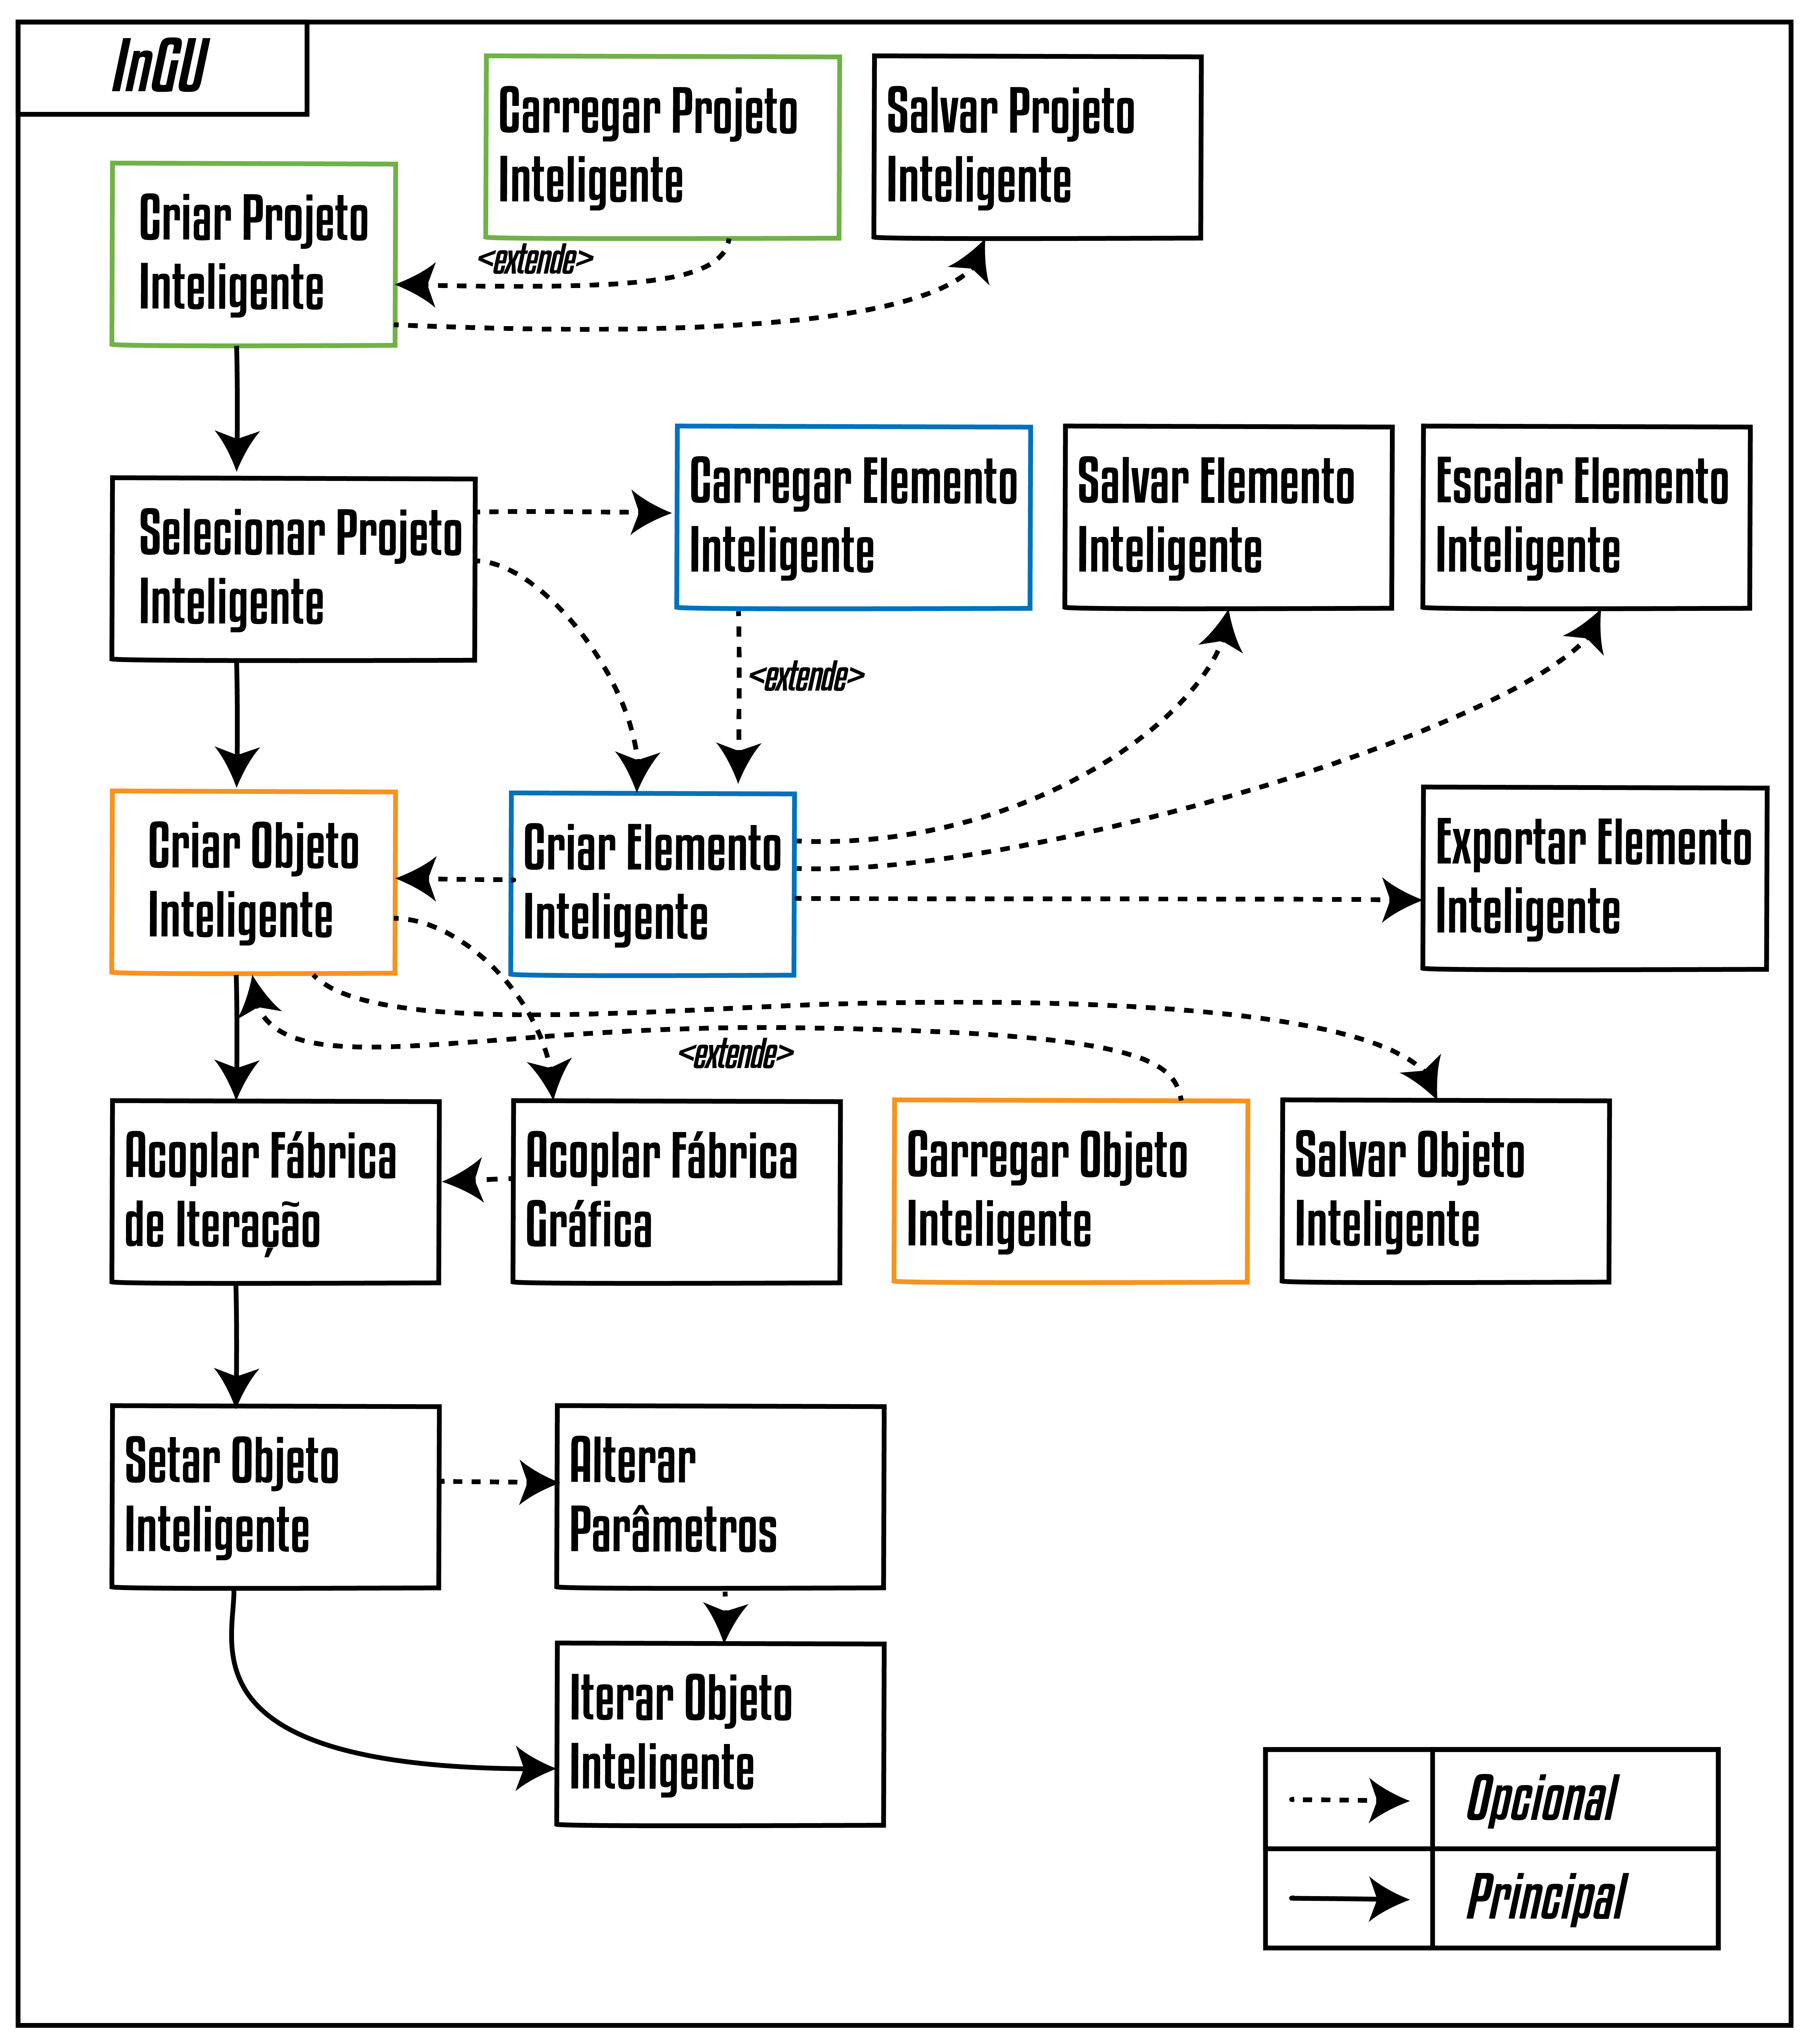
\includegraphics[width=\linewidth]{Figures/CasoDeUso@16x.png}
	\caption{Fluxo de caso de uso do ambiente computacional InGU, em azul as atividades de criação de elementos, em verde as atividades de criação de projetos e em laranja as atividades de criação de objetos.}
	\label{fig:caso_uso}
\end{figure}

Primeiramente, é necessário criar um projeto e selecioná-lo. Cada atividade representada no fluxograma é executada por um comando correspondente. O mesmo fluxo pode ser observado no Anexo~\ref{annex2}. As primeiras linhas de comando representadas neste arquivo são de criação de projetos.

Ao criar um objeto, seus elementos também são criados. Esta funcionalidade está disponível ao usuário uma vez que ele tenha selecionado um projeto. É possível ainda criar um objeto a partir de um elemento. Desta forma, há garantia da igualdade inicial entre os modelos.

Com um objeto criado corretamente é possível adicionar a ele uma fábrica de iteração e uma gráfica. Ao acoplar a fábrica de iteração o método iterativo é liberado, bem como a possibilidade de alterar os parâmetros do objeto.

Também existe a possibilidade de se exportar elementos, para elementos \textit{WiseGraphic} isso significa a exportação de imagem no formato \textbf{P}ortable \textbf{N}etwork \textbf{G}raphics, ou \textit{png}, com seu comando representado na linha $7$ do Anexo~\ref{annex2}.

Como mencionado anteriormente, a mesma estrutura foi utilizada na construção do ambiente computacional composto por elementos gráficos \textit{IGU}, conforme a Figura~\ref{fig:caso_uso2}.

\begin{figure}[!htbp]
	\centering
	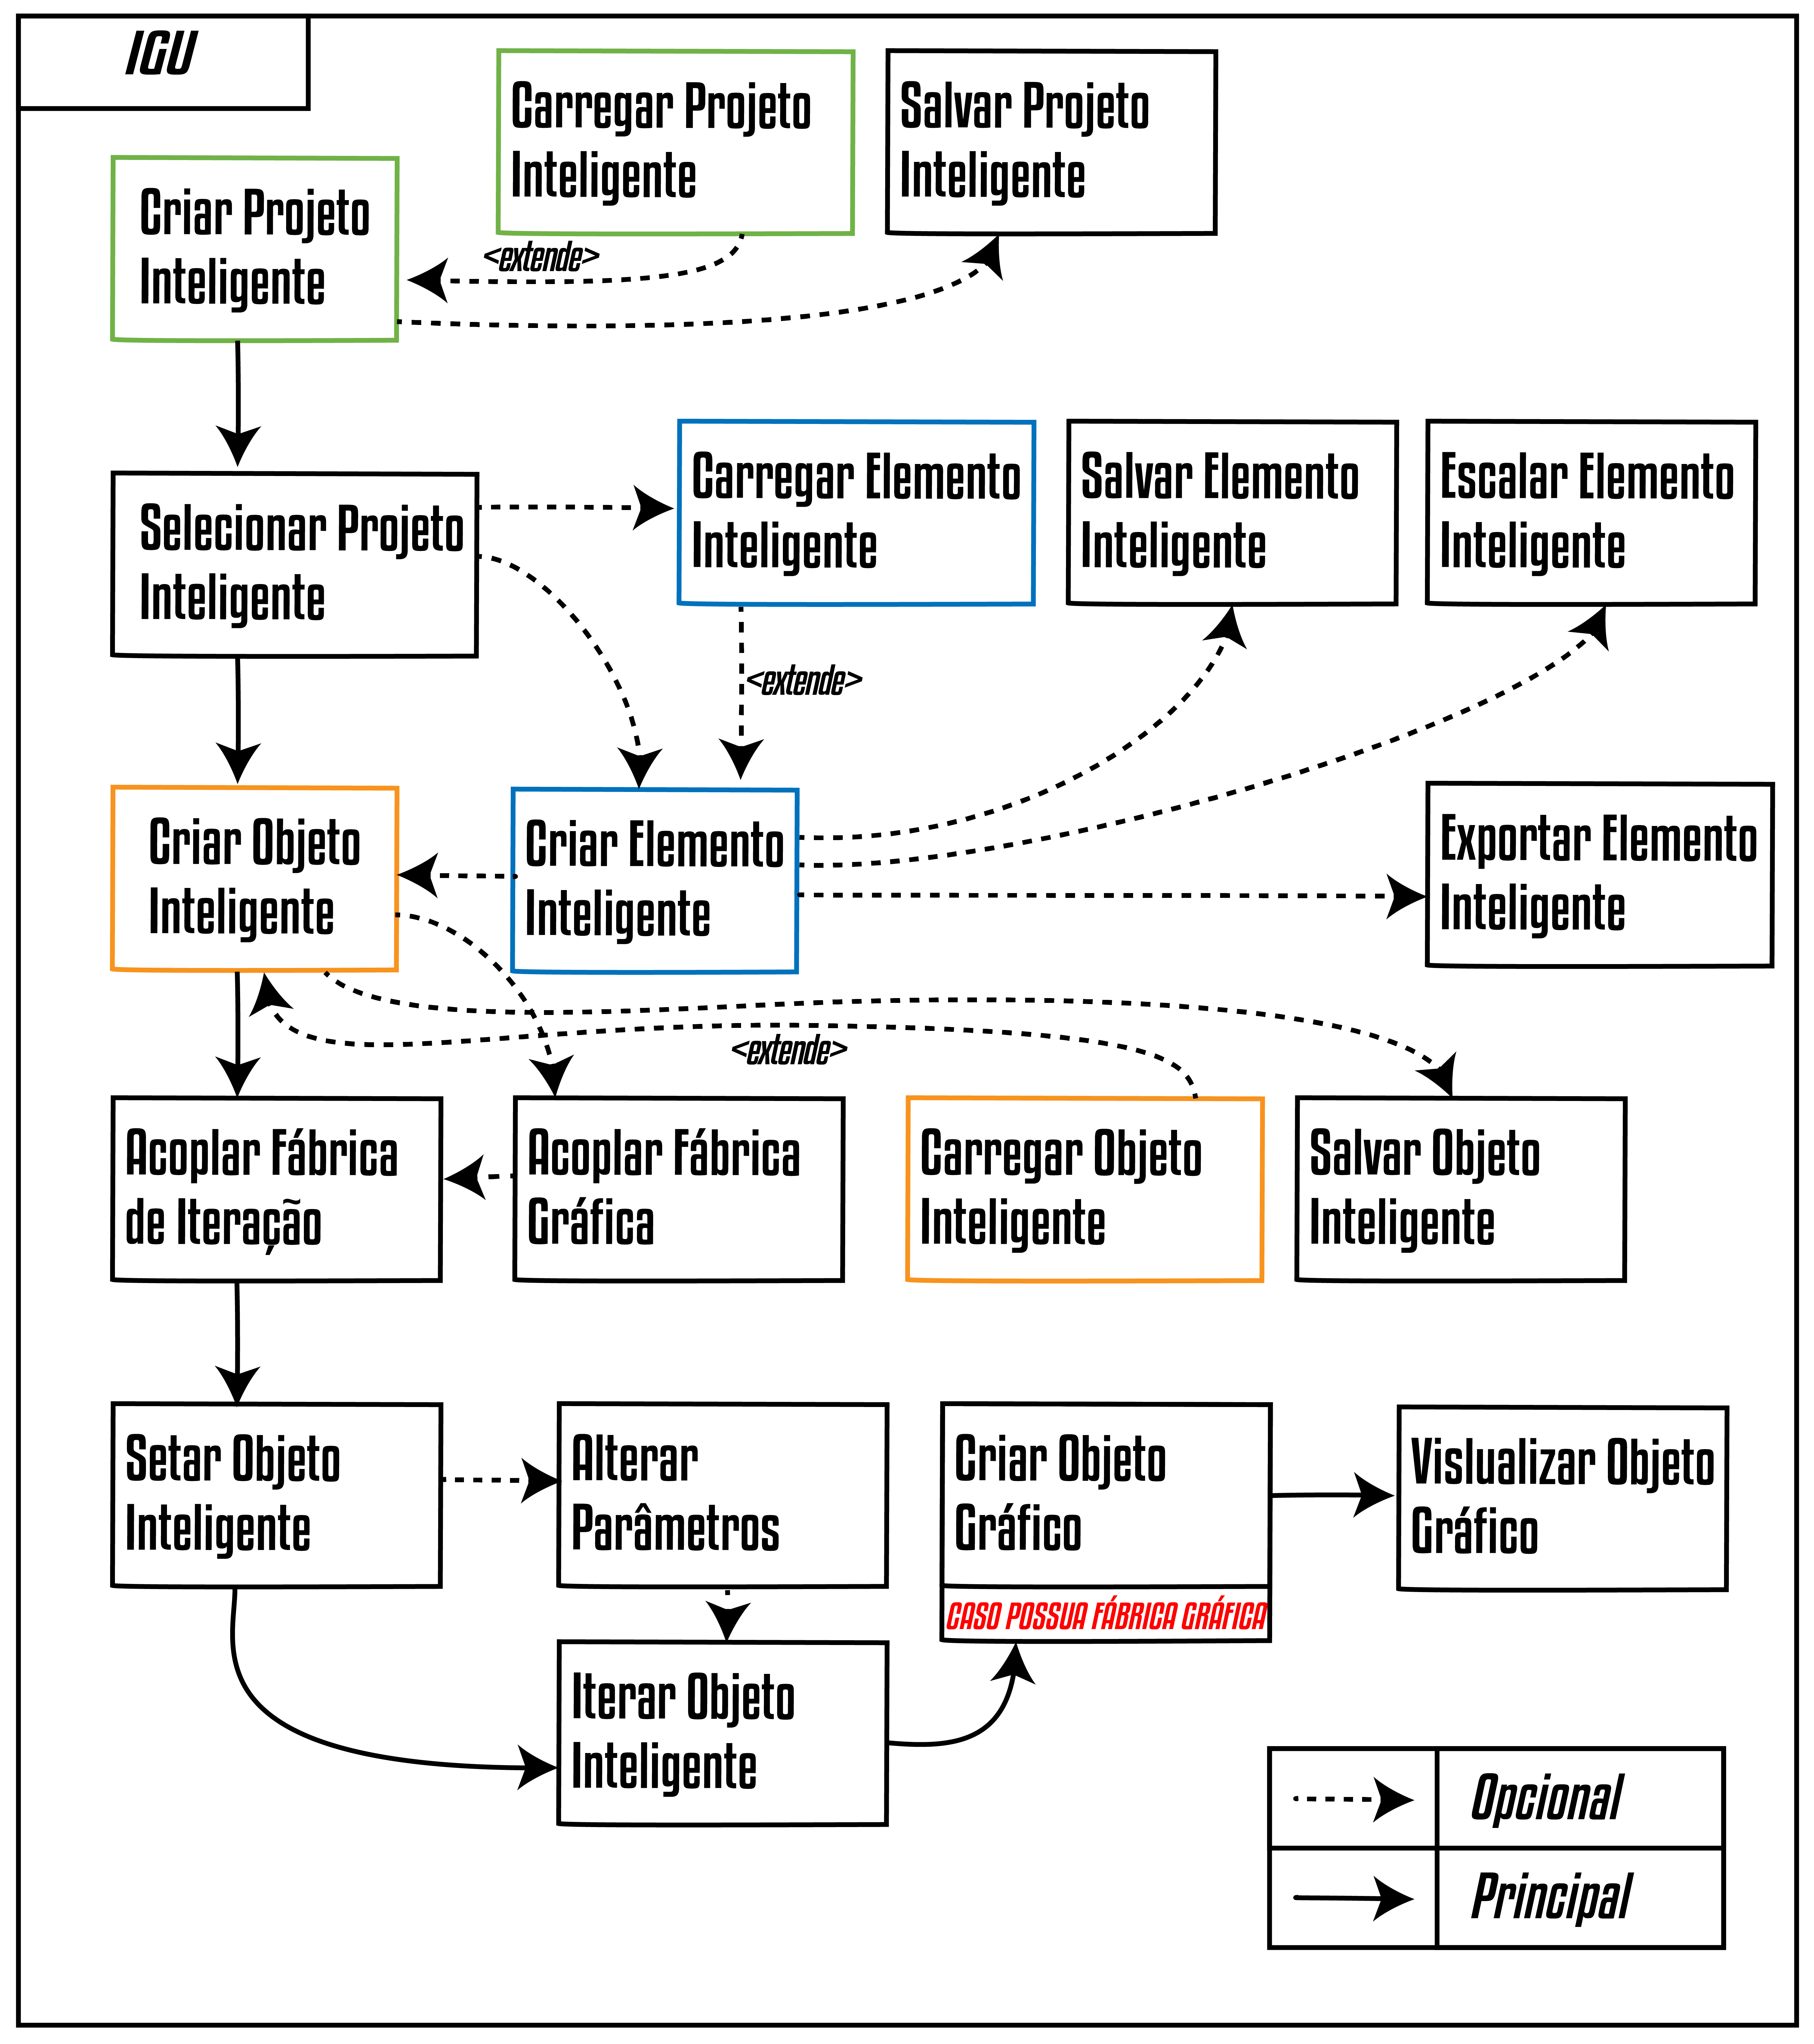
\includegraphics[width=\linewidth]{Figures/CasoDeUso2@16x.png}
	\caption{Fluxo de caso de uso do ambiente computacional IGU.}
	\label{fig:caso_uso2}
\end{figure}

Desta forma, o principal fluxo de uso da interface gráfica foi desenvolvido. O funcionamento apresentado pela Figura~\ref{fig:caso_uso2} difere do apresentado na Figura~\ref{fig:caso_uso} apenas na visualização dos objetos gráficos disponibilizada pelos elementos gráficos. Isto garante que ambos os ambientes computacionais sejam alterados em uma eventual atualização de código e que tenham funcionamento idêntico.

%--------------------------------------------------------------------------------%
\section{JANELA PRINCIPAL}\label{sec:janela}

O ambiente com interface gráfica foi nomeado de \textbf{I}terador \textbf{G}ráfico \textbf{U}niversal (IGU), que também está presente como parte de um projeto \textit{Qt}/\textit{C++}. Diferentemente do InGU, este possui elementos gráficos. O principal elemento gráfico disponibilizado pela interface gráfica é a janela principal, que é um objeto do tipo \textit{QMainWindow}. Estes objetos são disponibilizados pela biblioteca \textit{Qt} e permitem que um projeto \textit{C++} possua uma interface gráfica utilizando diretivas OpenGL e GLUT (\textit{The OpenGL Utility Kit})~\cite{OpenGL}.

\begin{figure}[!htbp]
	\centering
	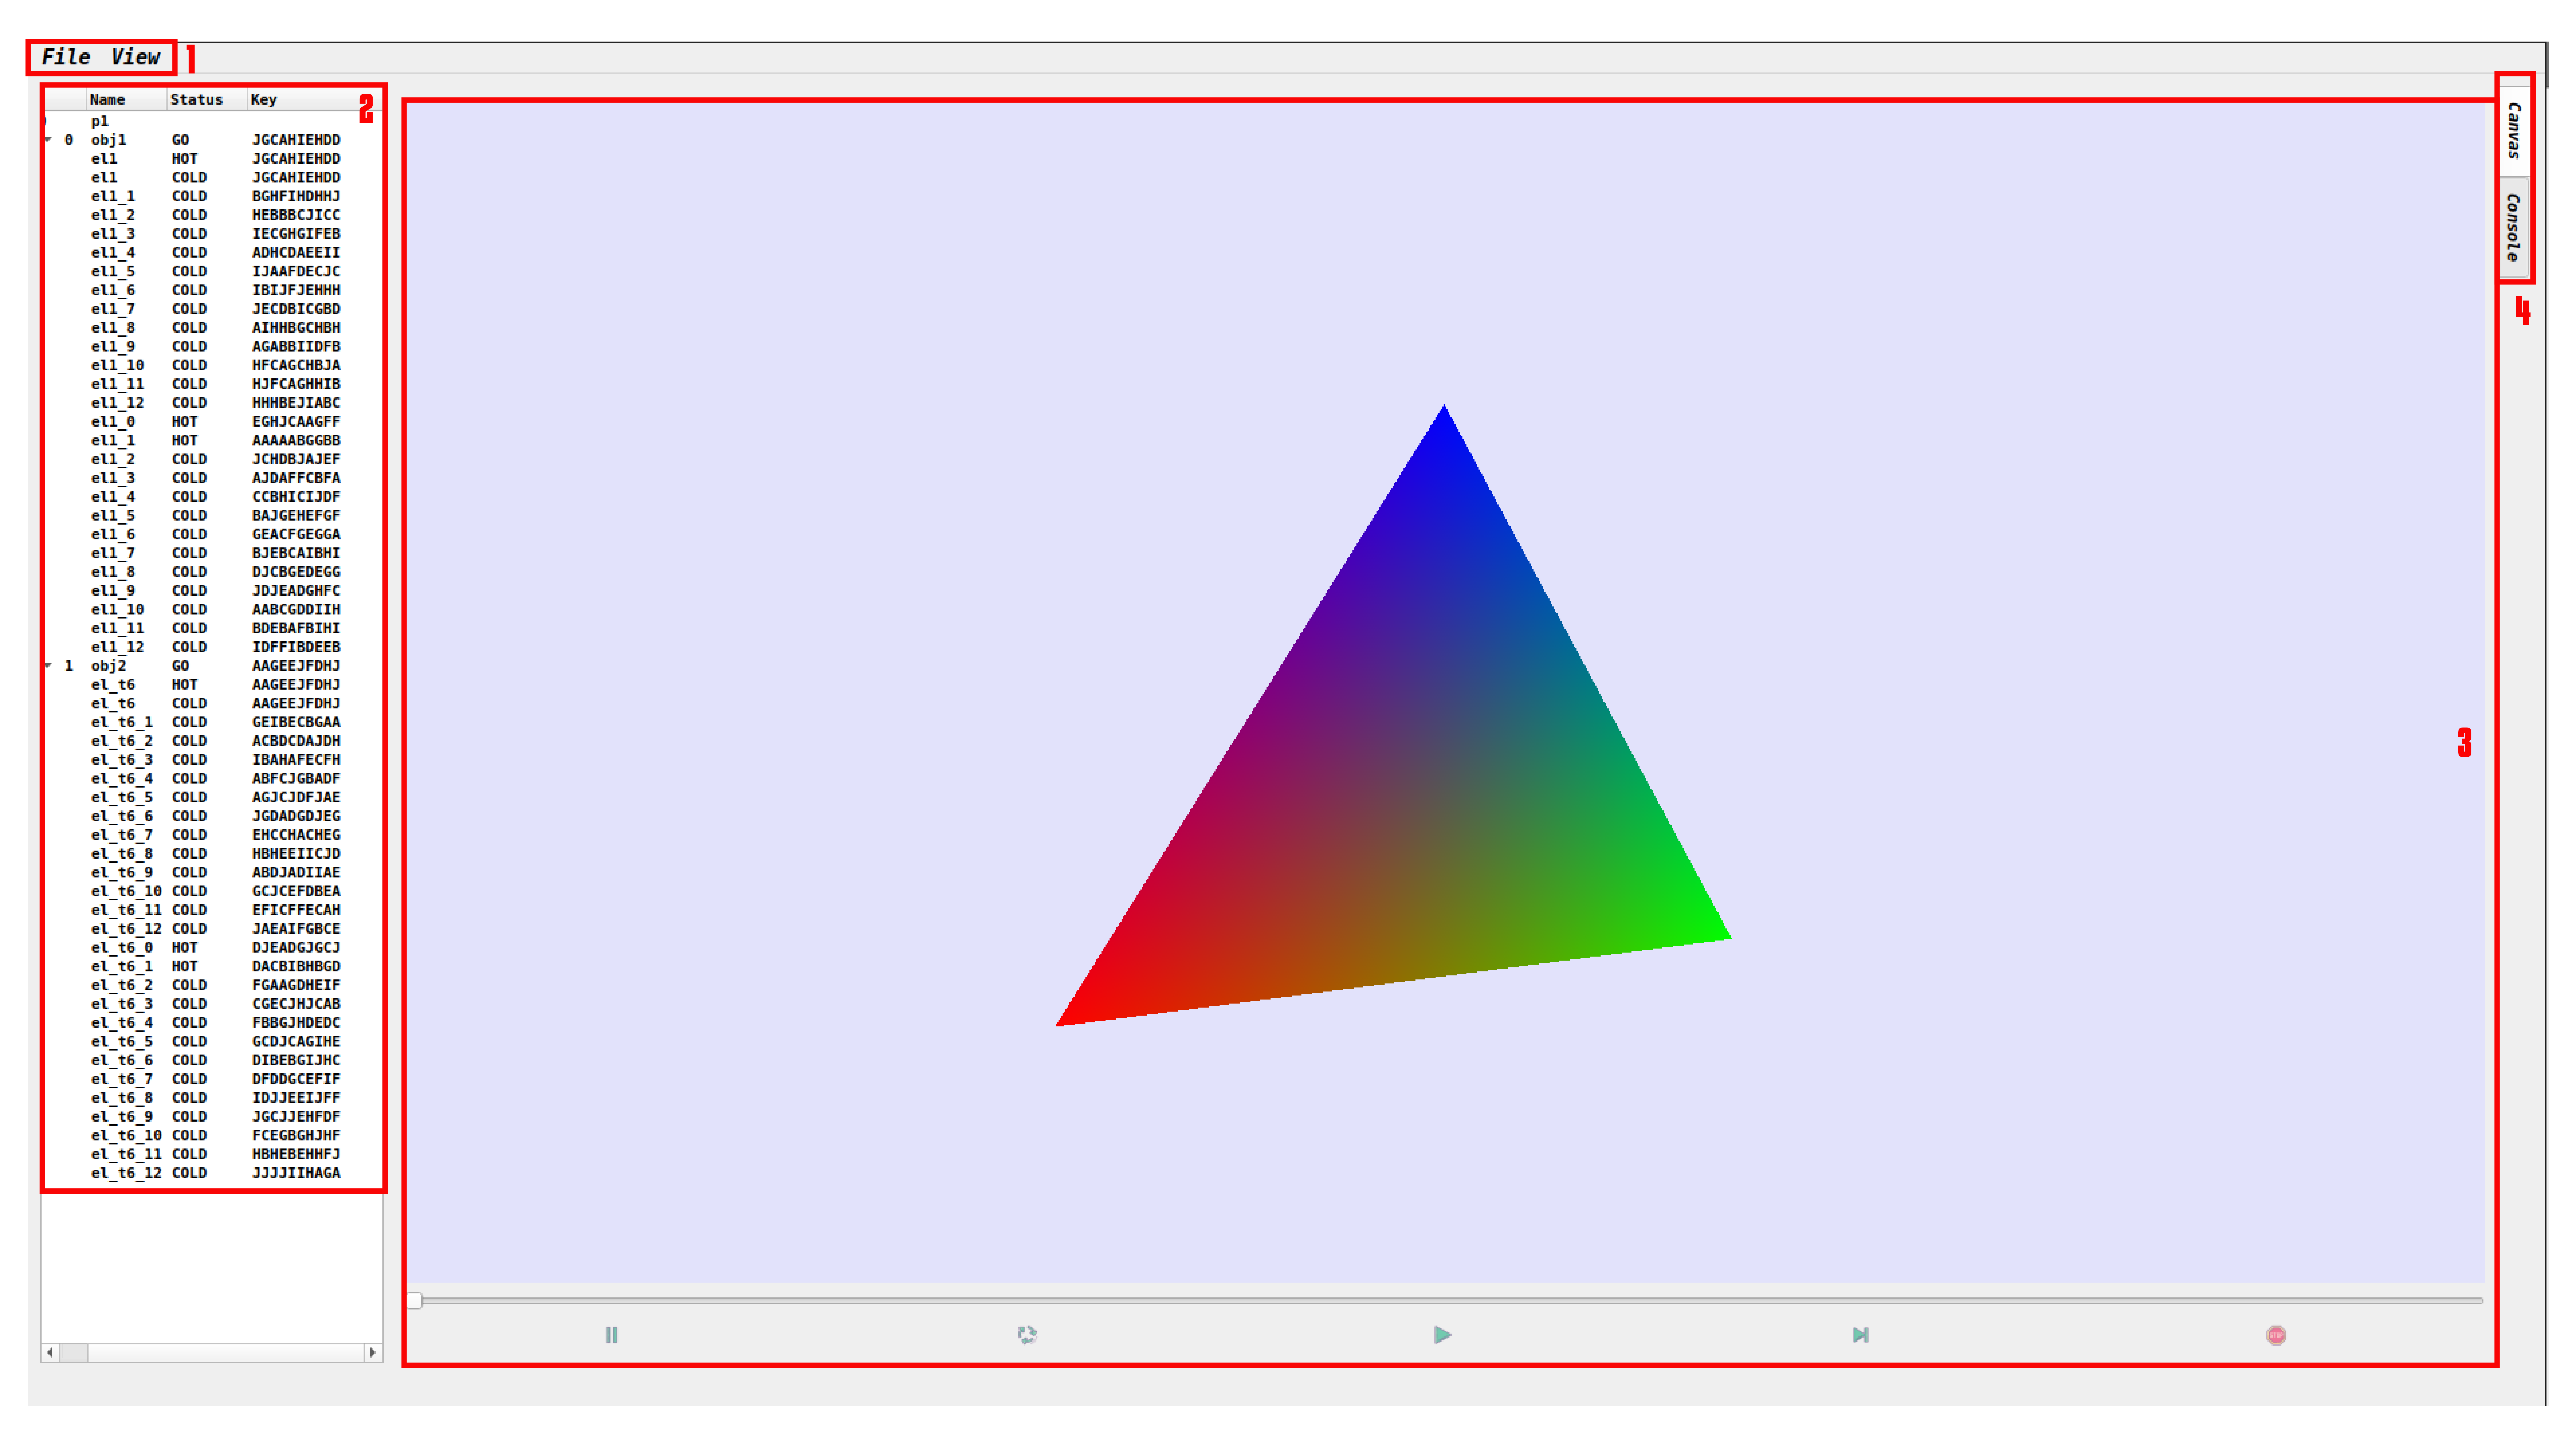
\includegraphics[width=\linewidth]{Figures/IGU_001a.png}
	\caption{Janela principal ambiente computacional IGU. Da esquerda para a direita: (A) Menu principal do programa; (B) Árvore de projetos e seus elementos; (C) Área de trabalho, no caso mostrando OpenGl \textit{Canvas}; (D) Seleção de abas}
	\label{fig:UI}
\end{figure}

A Figura~\ref{fig:UI} ilustra o comportamento inicial da ferramenta computacional. Ao ser aberta, o ambiente de trabalho, projetos, objetos e elementos são recuperados de um arquivo contido na mesma parte da ferramenta computacional. Este arquivo é salvo toda vez que a ferramenta é encerrada com projetos ainda no ambiente. Ainda nesta figura estão representados os principais grupos de elementos gráficos.

As próximas seções discorrem sobre cada grupo de elemento gráfico presente na janela principal da ferramenta e seu funcionamento.

%--------------------------------------------------------------------------------%
\subsection{MENU}\label{sec:menu}

O primeiro grupo são os elementos que constituem o menu principal da aplicação. Cada opção do menu é representada por um uma linha de texto, ao selecionar a linha uma ação é executada:

\begin{itemize}
	\item \textbf{Exit}: Fecha o ambiente computacional.
	\item \textbf{Jobs}: Abre a Janela que exibe os trabalhos criados.
	\item \textbf{Open Canvas}: Abre uma nova janela contendo um novo elemento gráfico OpenGL \textit{Canvas}.
\end{itemize}

\begin{figure}[!htbp]
	\centering
	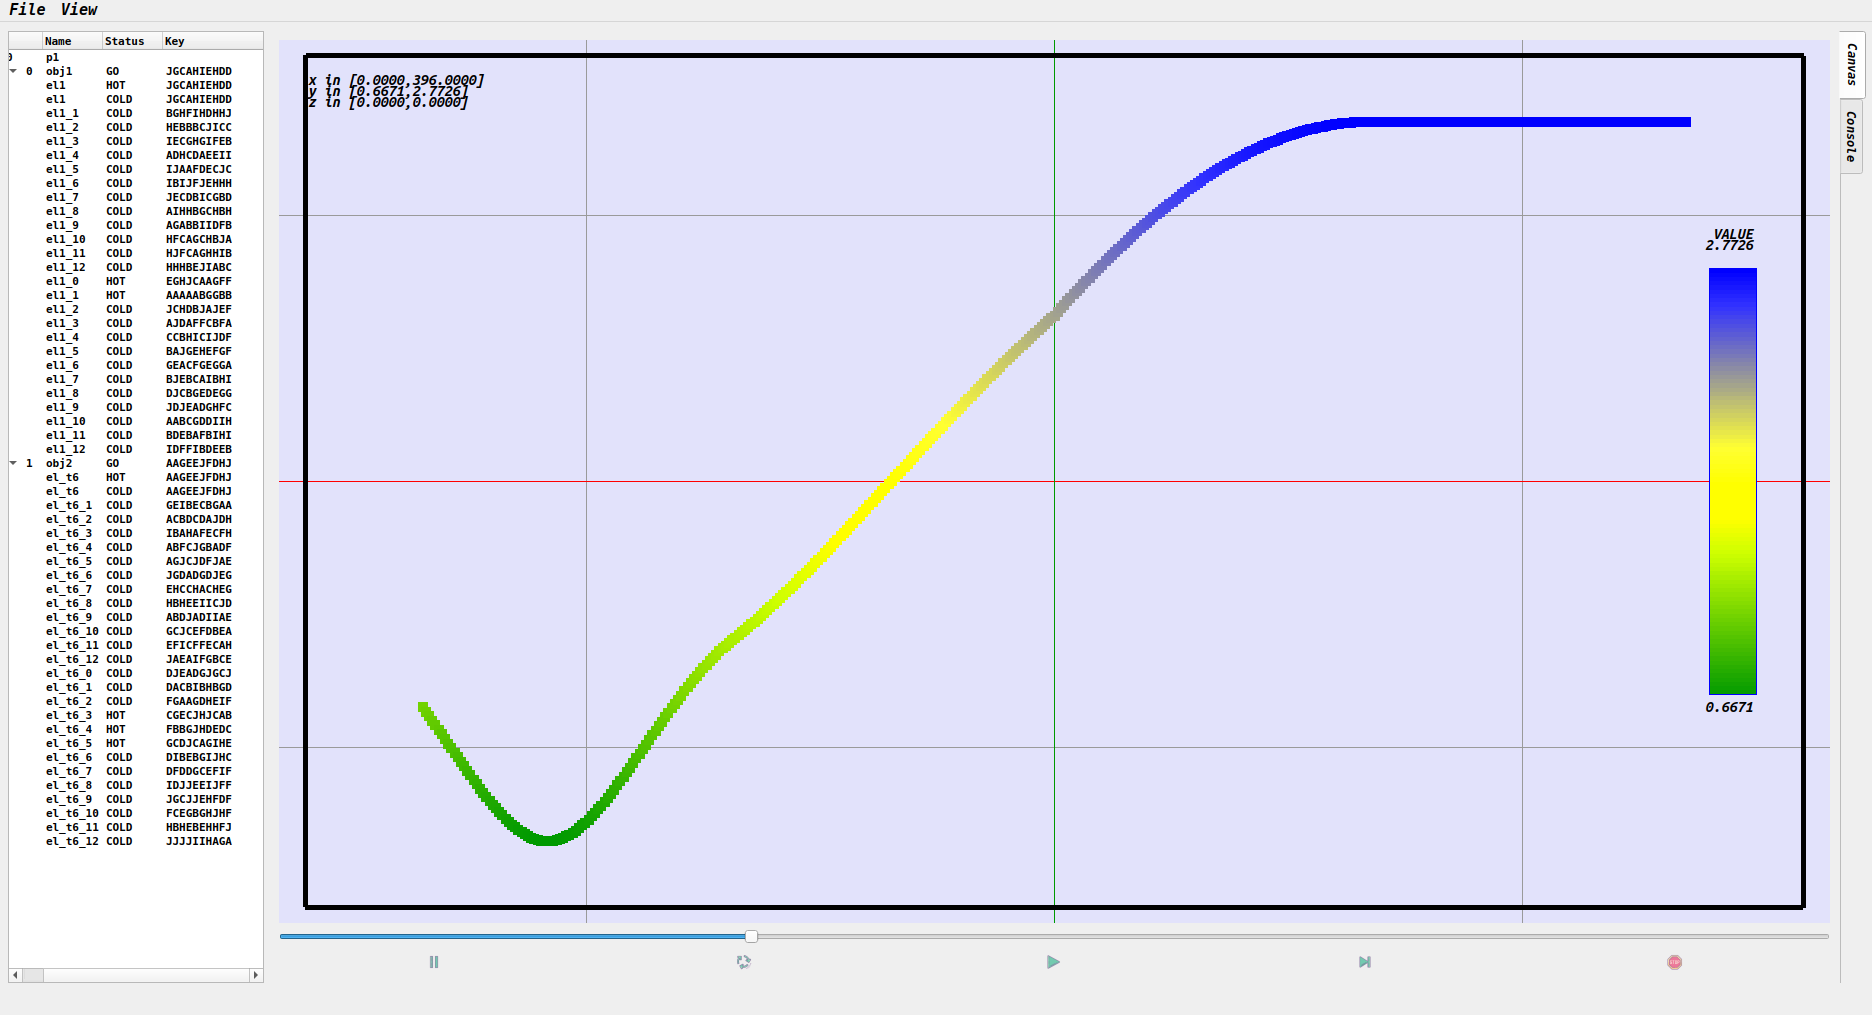
\includegraphics[scale=1]{Figures/IGU_016.png}
	\caption{Opções do menu principal da ferramenta computacional \textit{IGU}}
	\label{fig:menu}
\end{figure}

Ao abrir um novo elemento gráfico \textit{Canvas}, um novo nome será listado ao executar o comando para listar canvas. Isso possibilita que mais de um objeto seja exibido ao mesmo tempo em janelas distintas.

%--------------------------------------------------------------------------------%
\subsection{ABAS E ÁREA DE TRABALHO}\label{sec:abas}

As abas da janela principal selecionam o elemento de interface gráfica que é exibido na área de trabalho da aplicação.

\begin{figure}[!htbp]
	\centering
	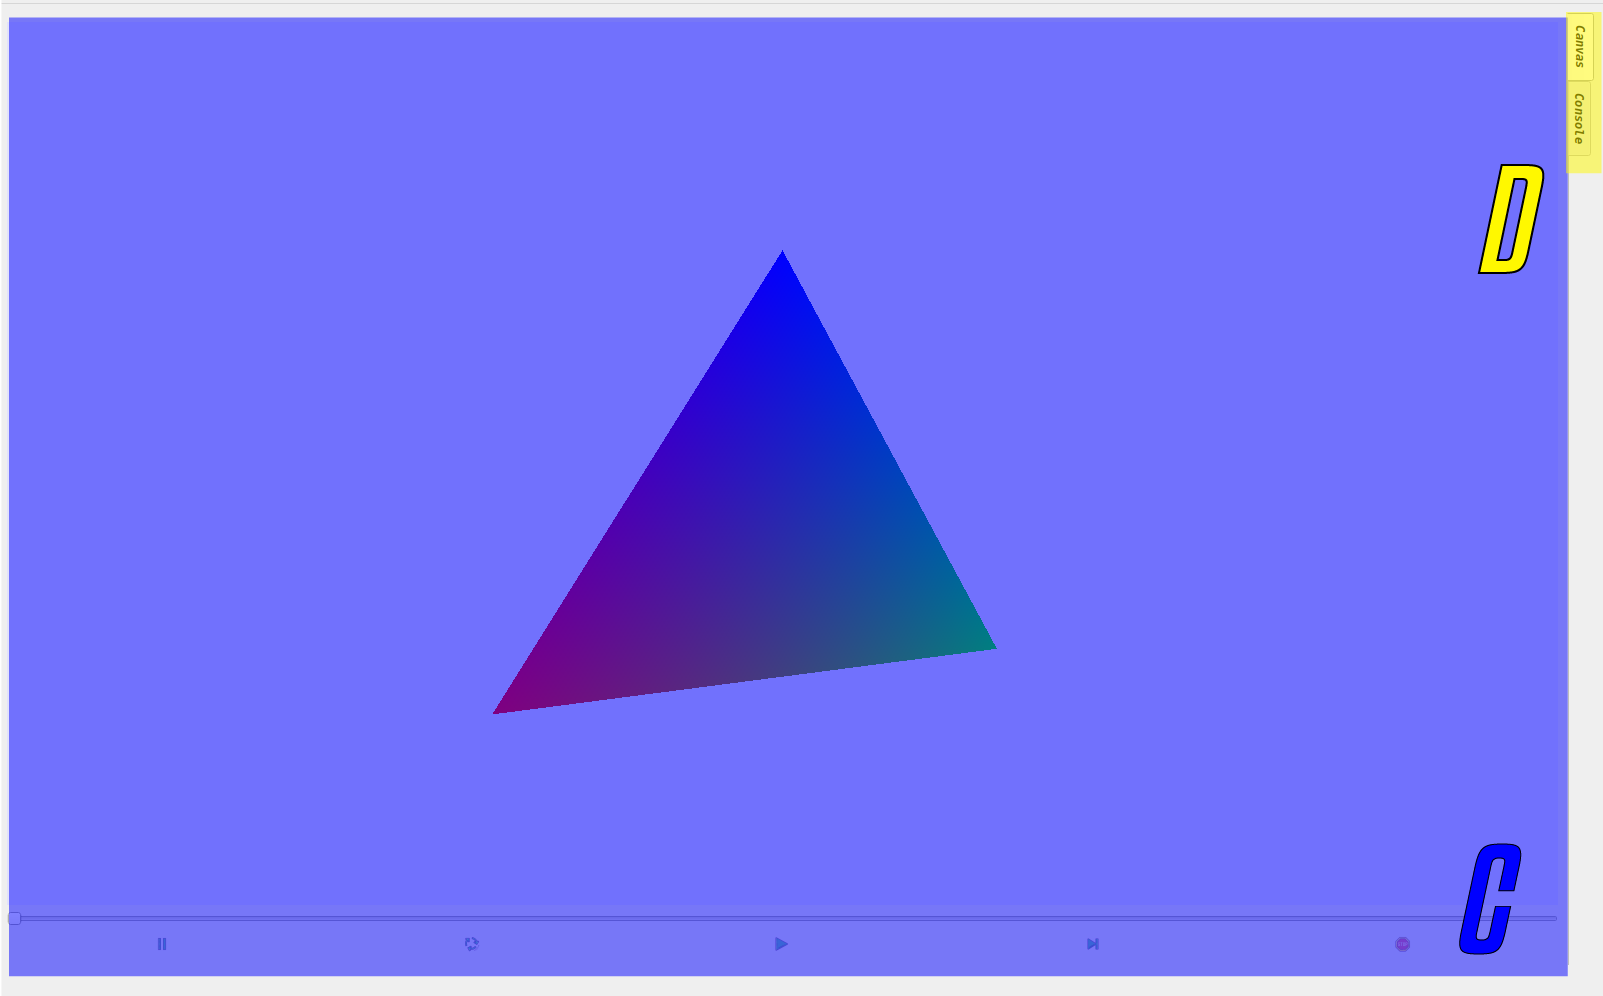
\includegraphics[width=\linewidth]{Figures/IGU_001a_34.png}
	\caption{Parte da janela principal contendo a área de trabalho e as abas que selecionam a interface selecionada, sendo os componentes: (C) Área de trabalho \textit{Canvas}; (D) Seleção de abas}
	\label{fig:abas}
\end{figure}

Ao selecionar uma das abas, os elementos de interface de usuário da área de trabalho são trocados. Estes elementos são objetos do tipo \textit{QWidget}, que por sua vez são divididos em dois ambientes: o \textit{Canvas} e o \textit{Console}. 

A aba \textit{Console} exibe um ambiente similar ao disponibilizado pelo ambiente \textit{InGU}. Utilizando um elemento de exibição textual longa, uma linha de texto como entrada e um botão, os mesmo comandos disponibilizados na Seção~\ref{sec:console} são acessados por estes elementos gráficos. Para executar uma linha de comando, basta inserir-lá no elemento gráfico e pressionar o botão ou a tecla \textit{Enter}, a resposta é acoplada ao elemento de exibição textual longa.

\begin{figure}
	\centering
	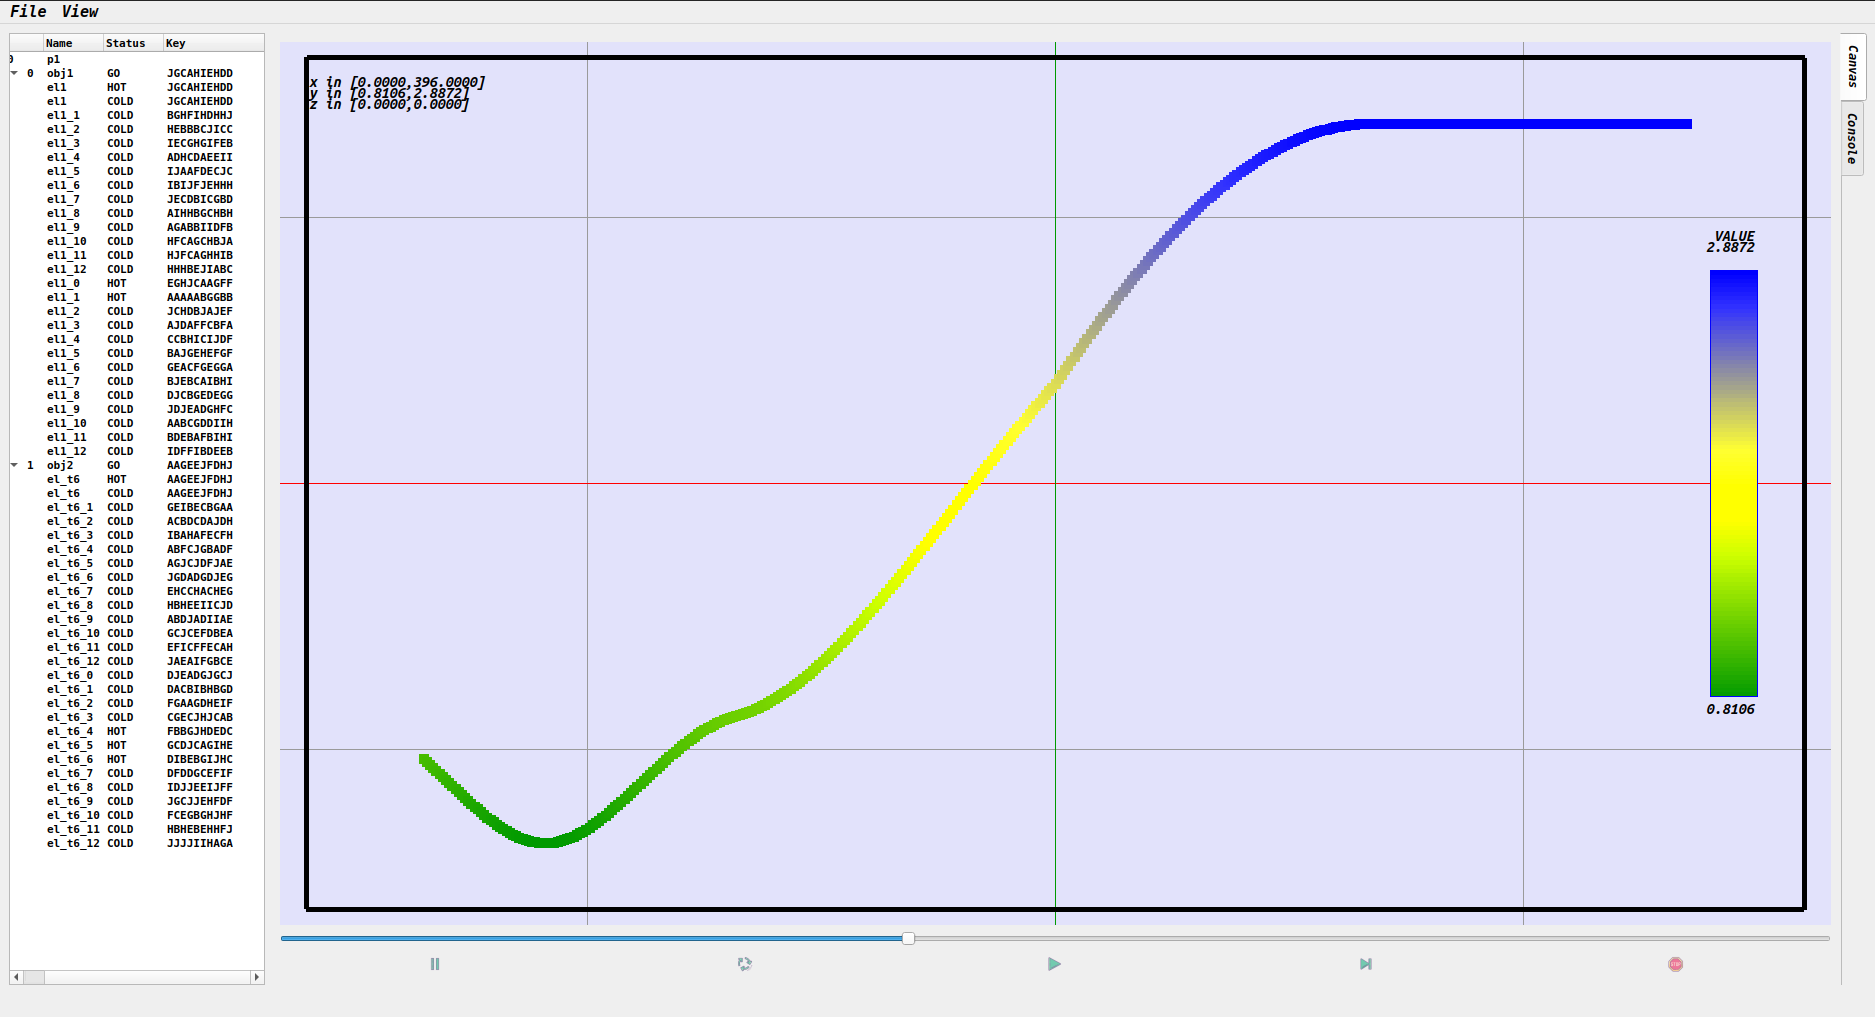
\includegraphics[width=.9\linewidth]{Figures/IGU_017.png}
	\caption{Área de trabalho exibindo o elemento gráfico \textit{Canvas} com a aba \textit{Canvas} selecionada.}
	\label{fig:sfig1}
\end{figure}

\begin{figure}
	\centering
	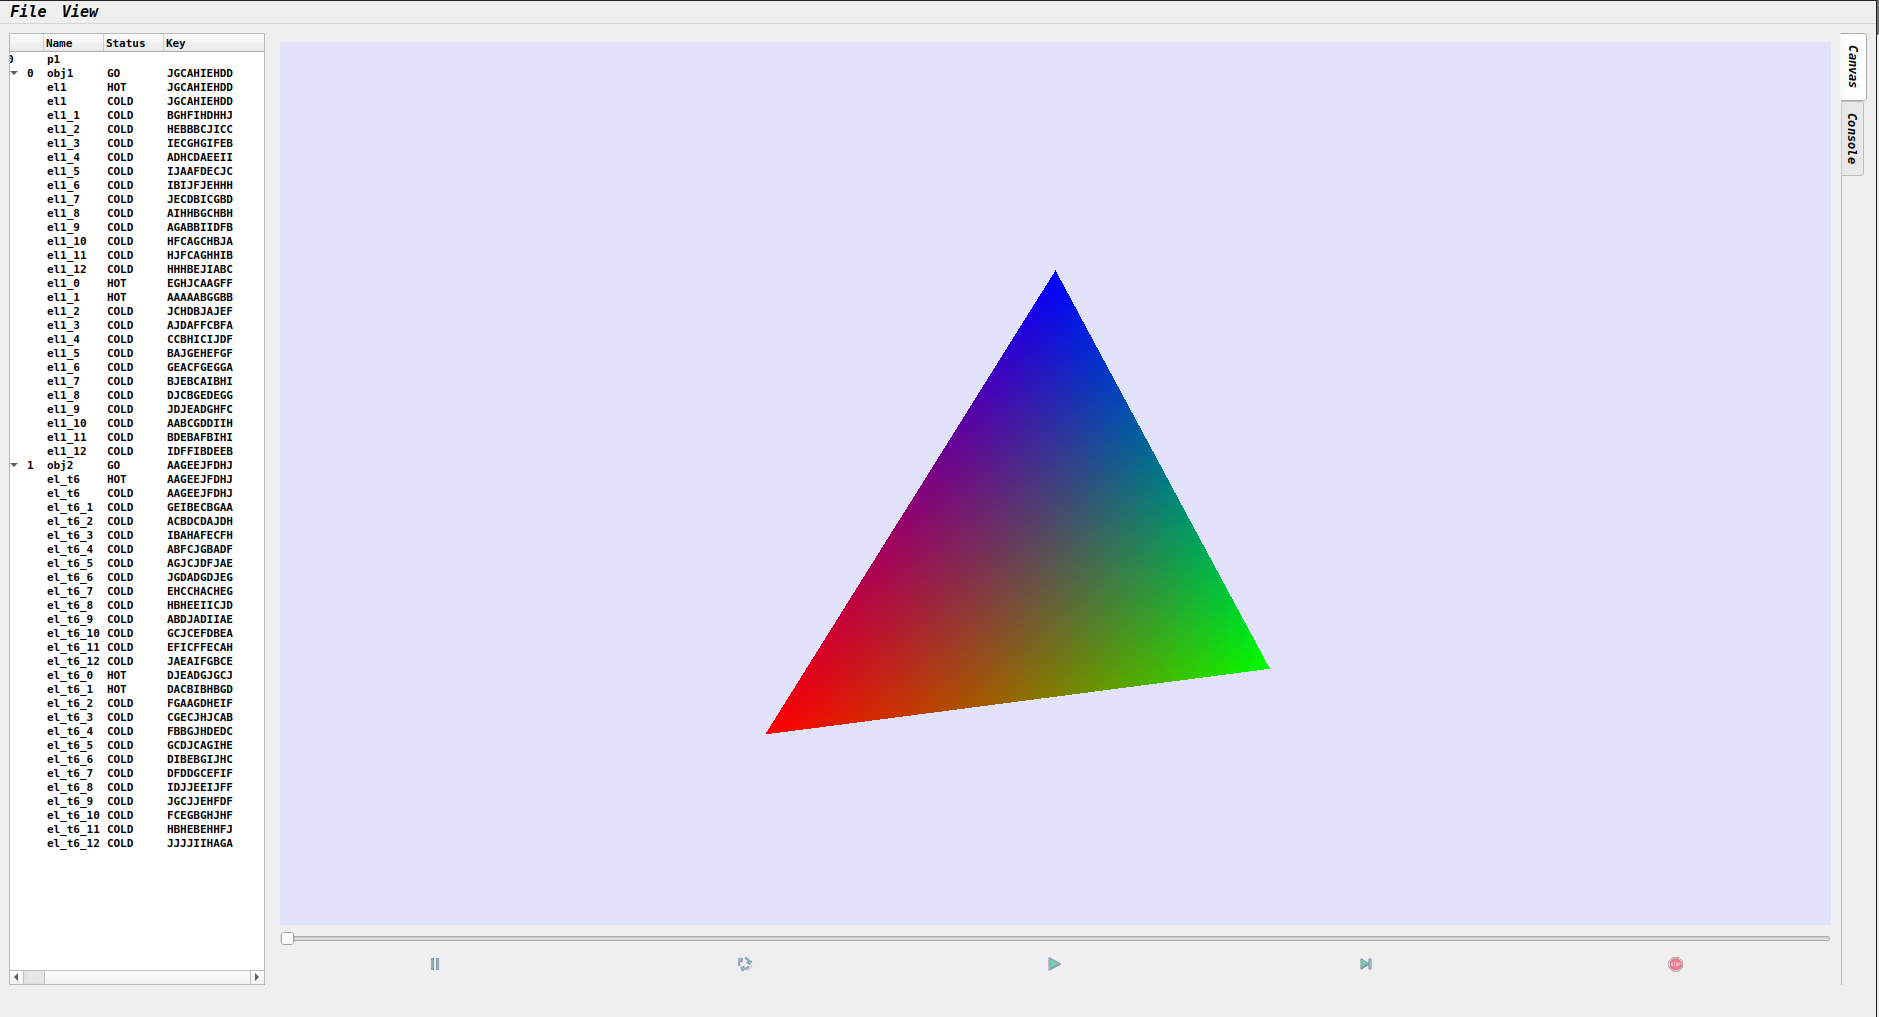
\includegraphics[width=.9\linewidth]{Figures/IGU_001.png}
	\caption{Área de trabalho exibindo o elemento gráfico \textit{Console} com a aba \textit{Console} selecionada.}
	\label{fig:sfig2}
\end{figure}

A Figura~\ref{fig:abas} mostra as áreas de trabalho disponibilizadas ao selecionar uma das abas. Através da opção \textit{Canvas}, o elemento gráfico que contém um \textit{QWidget} cuja principal função é uma tela \textit{OpenGL}. Os objetos gráficos, que são resultados de iterações, podem ser visualizados aqui. O funcionamento desta área de trabalho é descrito pela janela \textit{Canvas} e funciona como um 
reprodutor de vídeo.

As abas foram construídas para realizar todas as funções da ferramenta computacional com seus elementos gráficos. O ciclo de vida da \textit{thread} \textit{WiseThreadPool} esta diretamente ligado à interface gráfica. Ao utilizar a interface gráfica para percorrer os elementos gráficos, ou executar a animação, desencadeiam chamadas diretas as \textit{threads}.

%--------------------------------------------------------------------------------%
\section{ÁRVORE DE PROJETOS}\label{sec:arvore_projetos}

Além da área de trabalho, o elemento gráfico que exibe a árvore de projetos permanece fixo. Este elemento gráfico é um explorador de árvore \textit{QTreeWidget} que exibe todos os projetos carregados e suas estruturas. Esta árvore permite rapidamente verificar os elementos criados, seus nomes, suas chaves únicas e seu estado atual.

\begin{figure}[!htbp]
	\centering
	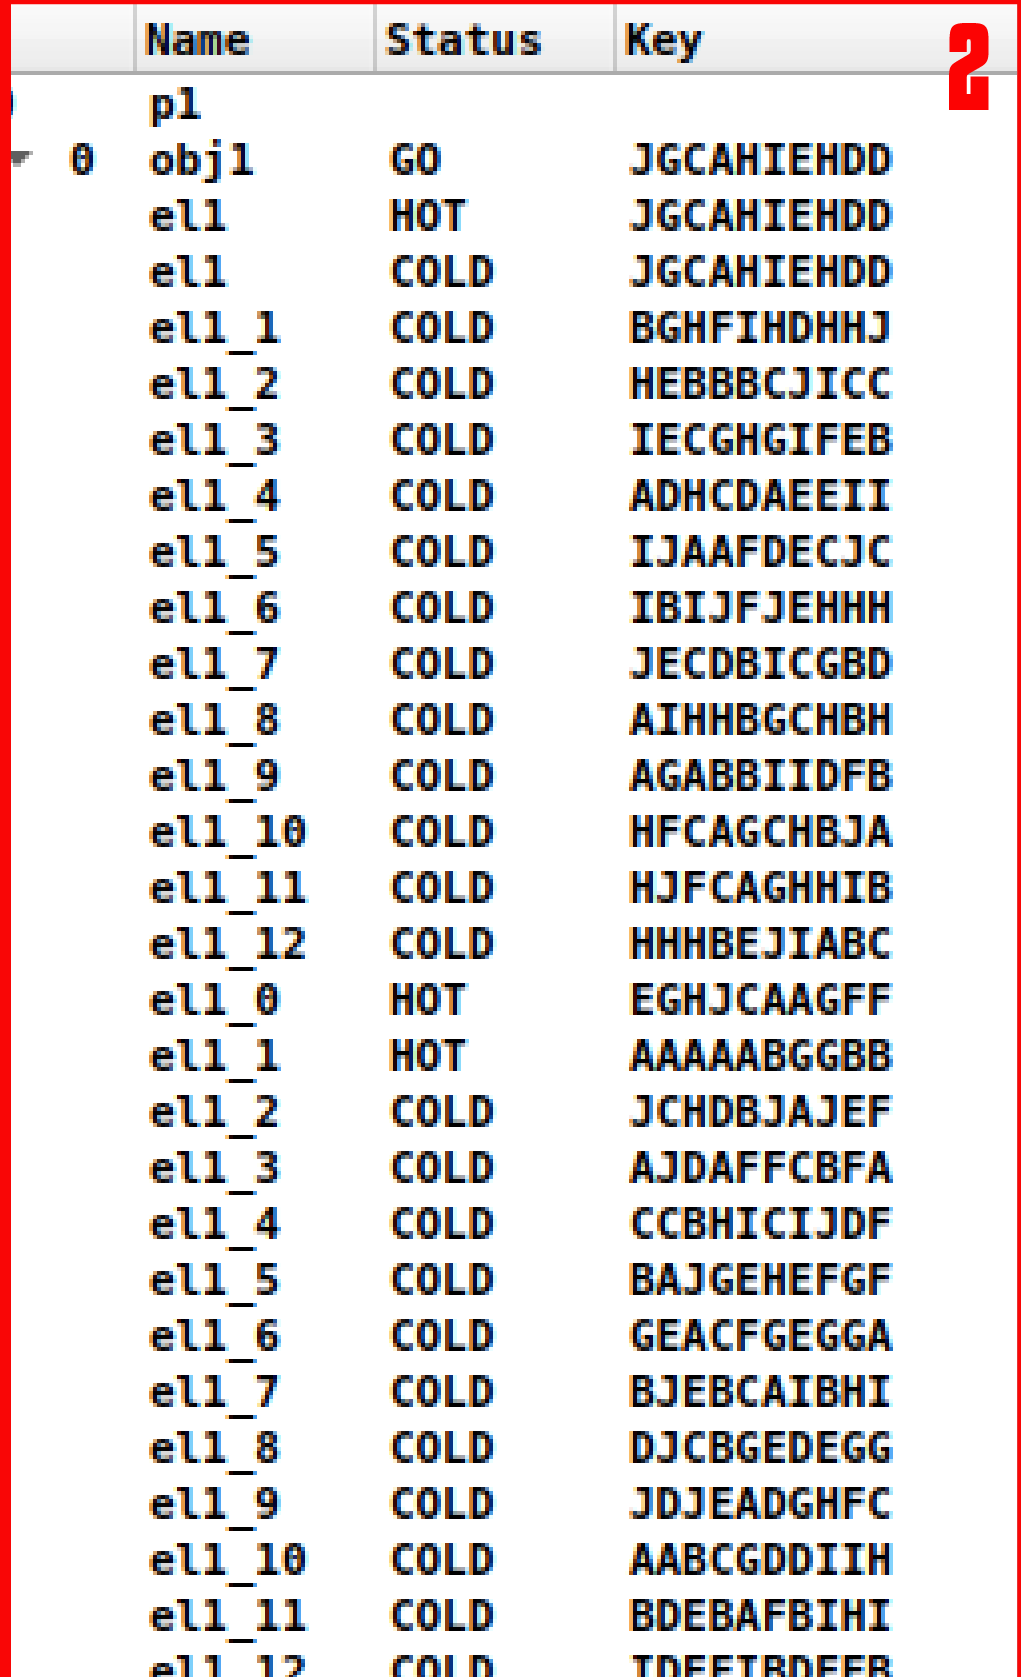
\includegraphics[width=0.4\linewidth]{Figures/IGU_001c.png}
	\caption{Árvore de projetos, na imagem a ferramenta apresenta um projeto $p1$, um objeto $obj1$ e seus elementos gráficos e elementos.}
	\label{fig:arvores}
\end{figure}

A Figura~\ref{fig:arvores} apresenta o elemento gráfico de uma árvore de projetos com objetos carregados. Na imagem está um projeto nomeado \textit{p1}, um objeto \textit{obj1} e diversos elementos e elementos gráficos. Como visto anteriormente quando o objeto está no estado \textit{GO} significa que ele já foi corretamente configurado e iterado. Dentro deste objeto estão os elementos e elementos gráficos. O primeiro elemento \textit{el1} é o elemento contido na estrutura \textit{Forno} e é o único elemento no estado \textit{Hot}. Em seguida, estão os elementos da estrutura \textit{Freezer}, seguidos pelos objetos gráficos.

Através da árvore de projetos é possível observar a troca de estado dos elementos, por exemplo, ao executar a animação, os elementos gráficos são sucessivamente aquecidos. Observa-se que a mesma quantidade de elementos gráficos e elementos, mantendo a consistência do objeto. Cada iteração gera um elemento com o resultado numérico e um elemento gráfico com a representação gráfica.

%--------------------------------------------------------------------------------%
\section{JANELAS}\label{sec:janelas}

Nesta seção, são descritas as janelas disponíveis no menu, o qual foi apresentado na Seção~\ref{sec:menu}. Existem dois tipos de janelas disponibilizadas pela ferramenta computacional: \textit{Canvas}, que funciona como um reprodutor de vídeo, exibindo elementos gráficos sucessivamente; \textit{Jobs}, o qual exibe todas as demandas criadas pelo programa enviadas à \textit{thread} inteligente \textit{WiseThreadTool}. Esta última janela pode ser instanciada apenas uma vez, enquanto diversos \textit{Canvas} podem ser disponibilizados e exibir diferentes objetos.

%--------------------------------------------------------------------------------%
\subsection{JANELA CANVAS}\label{sec:janela_canvas}

A janela e área de trabalho \textit{Canvas} possibilitam que o usuário selecione o quadro a ser exibido. Cada quadro representa um objeto do tipo \textit{GraphicObject} que é um componente do modelo gráfico \textit{GraphicModel}. O quadro é selecionado através de uma barra de progresso e de botões que alteram a animação feita com o objeto gráfico. Estes botões são:

\begin{itemize}
	\item \textit{Pause}: Pausa a animação do objeto gráfico;
	\item \textit{Repeat}: Este botão tem um funcionamento liga e desliga. Ao ser ligado, quando a animação chegar ao último elemento gráfico retornará ao primeiro;
	\item \textit{Play}: Este botão também tem um funcionamento liga e desliga. Ao ser ligado, o elemento gráfico irá percorrer por todos os quadros da animação;
	\item \textit{Avançar quadro}: Avança um quadro da animação;
	\item \textit{Stop}: Caso o \textit{Play} esteja ativo, ele é desativado e a tela volta ao primeiro elemento gráfico da animação.
\end{itemize}

Todas as funções do \textit{Canvas} só são disponibilizadas ao usuário depois que um objeto gráfico é ligado a tela \textit{OpenGl}. Quando um objeto é exibido em um \textit{Canvas}, cada quadro exibido altera quais objetos gráficos \textit{GraphicObject} estarão no estado aquecido \textit{Hot}. Isto foi feito utilizando a conexão entre objetos \textit{QObjects} e os elementos gráficos \textit{QWidget}. Desta forma a tela é capaz de acionar diretamente a estrutura do \textit{WiseThreadPool} e selecionar quais elementos devem ser aquecidos e exibidos. A mesma conexão é responsável por enviar a linha de comando da aba \textit{Console} a \textit{WiseThreadPool} para que seja executada e, em seguida, enviar a mensagem de resposta ao elemento textual.

\begin{figure}[!htbp]
	\centering
	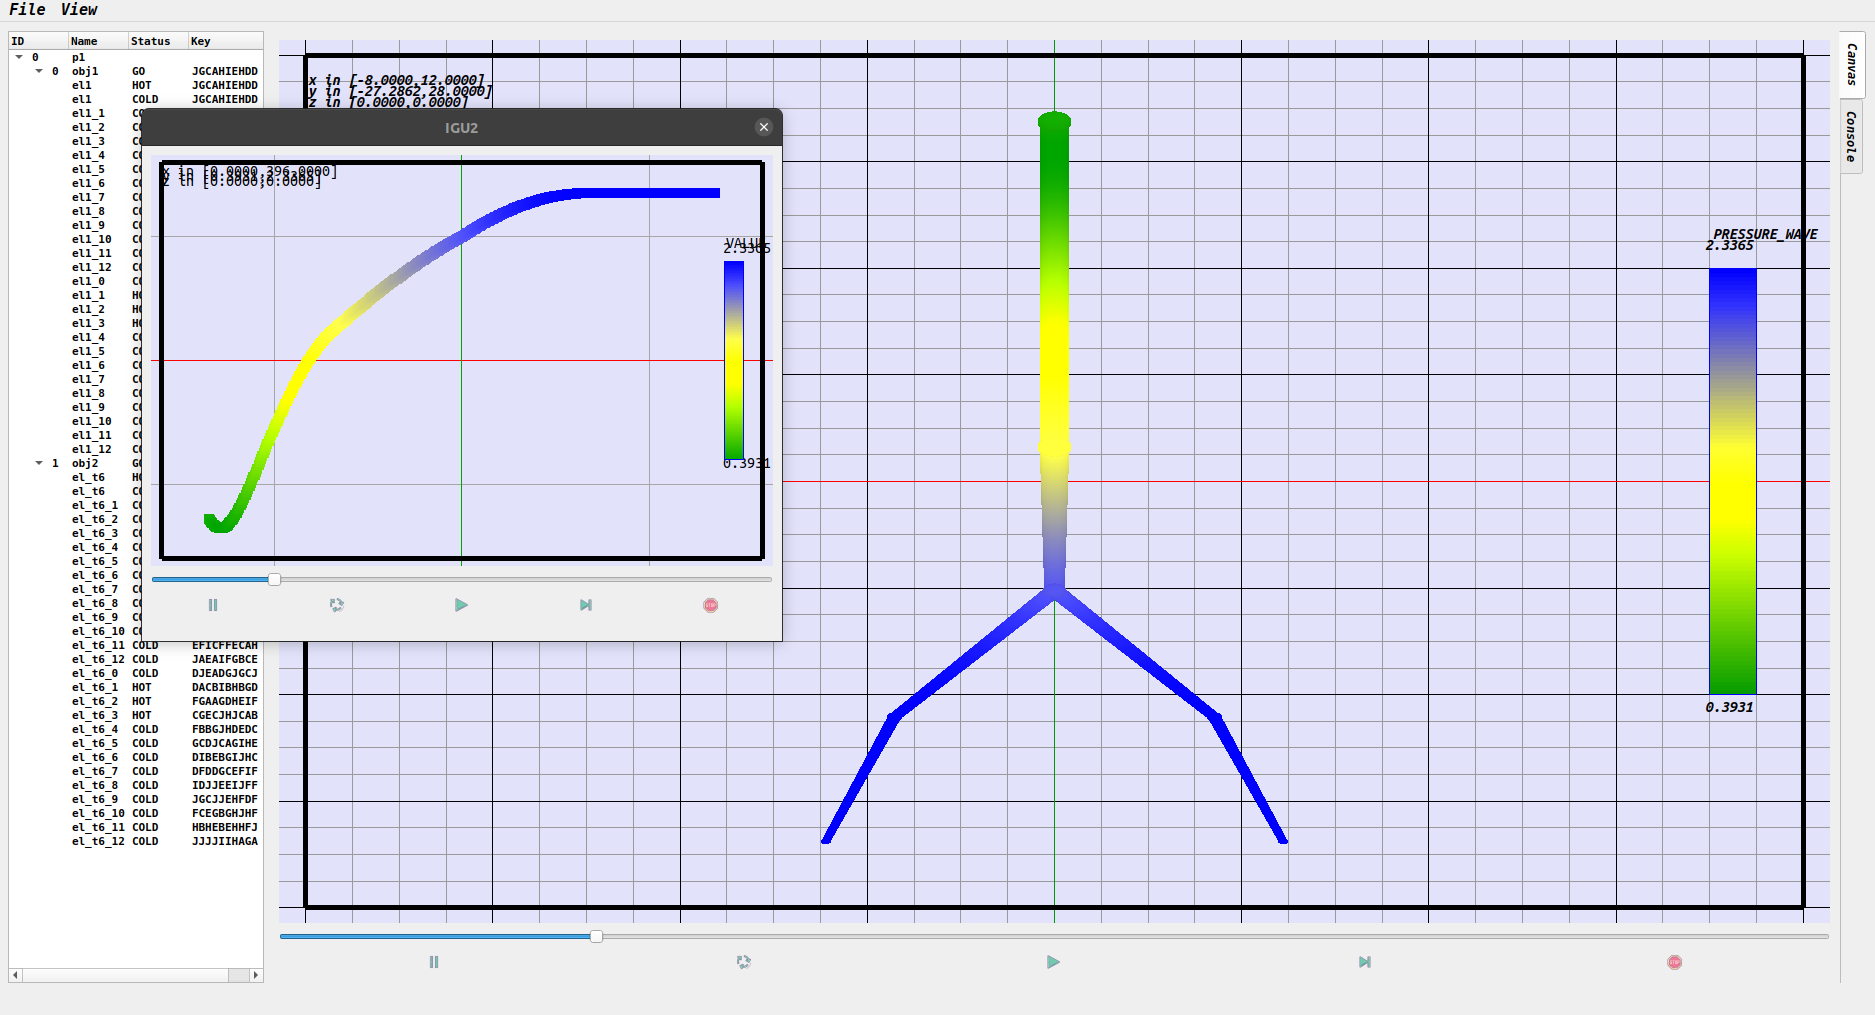
\includegraphics[width=\linewidth]{Figures/IGU_025.png}
	\caption{Ilustra a janela \textit{Canvas} exibida sobre a área de trabalho \textit{Canvas}, a janela exibindo um gráfico obtido como resultado e a área de trabalho exibindo a árvore arterial estudada.}
	\label{fig:canvas}
\end{figure}

Durante sua execução esta janela irá selecionar o elemento gráfico \textit{GraphicElement} que deve ser exibido, selecionando o elemento através do objeto gráfico \textit{GraphicObject}. Para que o elemento seja exibido corretamente ele precisa estar no estado \textit{Hot}, que representa o momento em que o elemento está corretamente carregado em memória com o modelo geométrico e o parâmetro a ser exibido. Portanto, ao selecionar o elemento o \textit{Canvas} irá criar trabalhos de aquecimento dos elementos. A coleção de objetos gráficos \textit{GraphicModel} é encarregada de enviar estes trabalhos a \textit{thread} inteligente \textit{WiseThreadPool}.

%--------------------------------------------------------------------------------%
\subsection{JANELA JOBS}\label{sec:janela_jobs}

A janela \textit{Jobs} exibe uma listagem compreensiva dos processos iniciados e enviados a \textit{thread} \textit{WiseThreadPool}. Cada comando executado via \textit{Console} ou elemento de interface gráfica irá gerar processos listados nesta janela.

\begin{figure}[!htbp]
	\centering
	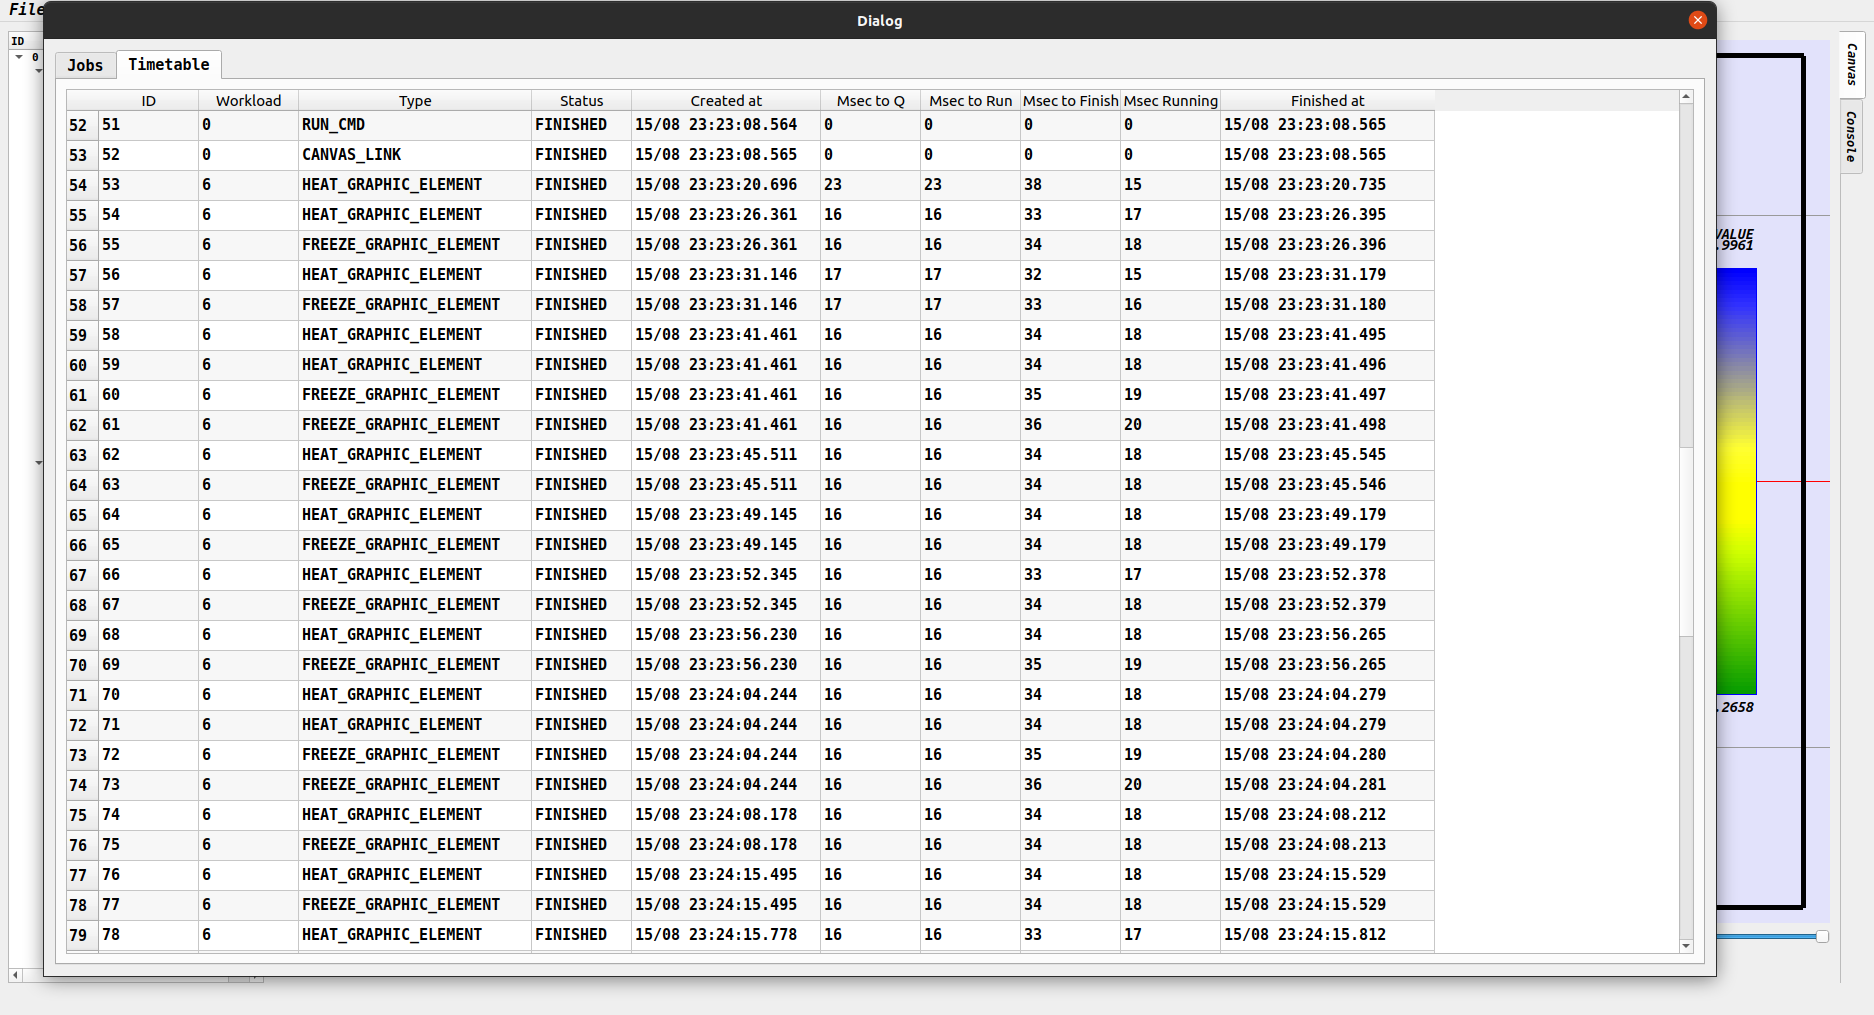
\includegraphics[width=\linewidth]{Figures/IGU_023.png}
	\caption{Janela \textit{Jobs} exibida com a aba \textit{Timetable} selecionada, a janela lista os trabalhos recebidos pela estrutura \textit{WiseThreadPool} e seus tempos de execução.}
	\label{fig:jobs}
\end{figure}

A Figura~\ref{fig:jobs} mostra a lista de todos os trabalhos recebidos pela \textit{thread} \textit{WiseThread} e suas propriedades. Cada linha nesta janela representa um \textit{WiseJob} e as colunas descrevem propriedades de cada trabalho:

\begin{itemize}
	\item \textit{ID}: Número de identificação;
	\item \textit{Workload}: Número da carga de trabalho;
	\item \textit{Status}: Estado do trabalho;
	\item \textit{Created at}: Data de criação;
	\item \textit{Msec to Q}: Milisegundos do momento da criação até a chegada a fila;
	\item \textit{Msec to Run}: Milisegundos do momento da criação até a alocação do trabalho em uma \textit{thread};
	\item \textit{Msec to Finish}: Milisegundos do momento da criação até o final de sua execução;
	\item \textit{Msec Running}: Milisegundos em execução;
	\item \textit{Finished at}: Data de finalização;
\end{itemize}

\begin{figure}[!htbp]
	\centering
	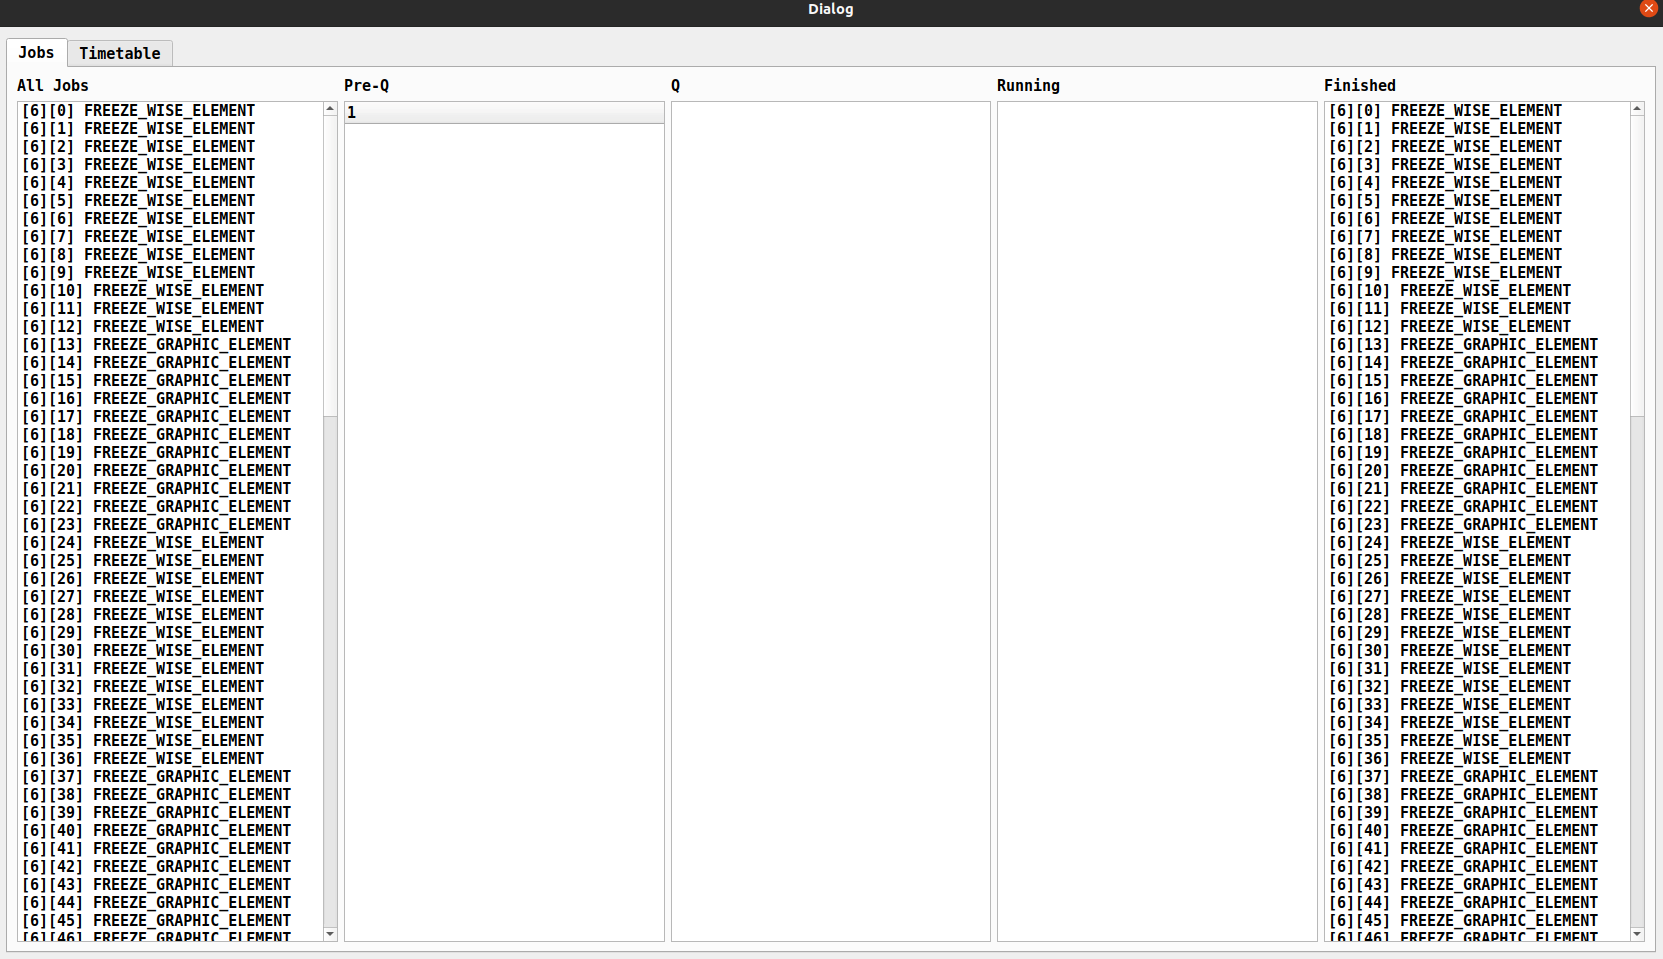
\includegraphics[width=\linewidth]{Figures/IGU_022.png}
	\caption{Janela \textit{Jobs} exibida com a aba \textit{Timetable} selecionada, a janela lista os trabalhos recebidos pela estrutura \textit{WiseThreadPool} e os separa logicamente pelas listas de espera.}
	\label{fig:jobs2}
\end{figure}

A Figura~\ref{fig:jobs2} demonstra as cinco listas exibidas ao selecionar a aba \textit{Timetable} da janela \textit{Jobs}. A primeira lista \textit{All Jobs} lista todos os trabalhos criados e as listas subsequentes listam as listas presentes no gerenciador de threads \textit{WiseThreadPool} descritas na Seção~\ref{sec:trabalhos}. Desta forma é possível verificar os trabalhos que aguardam execução, estão sendo executados ou foram finalizados.